\part{风湿性疾病急诊}

\chapter{系统性红斑狼疮}

系统性红斑狼疮(systemic lupus
erythematosus,SLE)是一种累及全身多系统多器官的自身免疫性疾病,其临床表现多种多样,血清内可出现多种自身抗体,为自身免疫病的原型。本病病程以病情缓解和急性发作交替为特点,有内脏(肾、中枢神经)损害者预后较差。女性多见,尤其是20~40岁的育龄女性。病程急性发作中可出现危及生命的急危重症,称为狼疮危象(lupus
crisis)。因涉及各个学科及专业,极易导致漏诊和误诊,应予以重视。

\subsection{病因与发病机制}

\subsubsection{病因}

病因尚未完全阐明,可能是遗传、环境、免疫及内分泌等多方面、复杂因素共同作用的结果,其主要特征是机体出现各种免疫反应异常。

\paragraph{遗传}

该病有较强的家族聚集性,患者一级亲属的患病率明显高于其他人。同时,家系调查还发现,SLE可以与其他自身免疫性疾病如自身免疫性溶血性贫血、甲状腺炎等同时存在。单卵双生疾病发生的一致率大约25\%~50\%,而双卵双生发病一致率为5\%左右。据计算至少4段染色体基因与SLE的发病密切相关,每一基因各自影响到SLE发病的中间环节,如免疫调节、蛋白降解、肽跨膜转运、免疫反应,补体激活等等。研究发现SLE患者与HLA-DR2、DR3,补体C\textsubscript{1q}
、C\textsubscript{2} 、C\textsubscript{4}
,以及部分非HLA基因编码的MBP、TNFα、IL-6、TCR、FcγR等相关。这些均表明遗传因素在易患人群中具有极其重要的作用,然而,很多SLE病例为散发,没有明确的遗传倾向,由此提示可能还有多种环境因素或者其他未知因素也参与了疾病的发生发展过程。此外,狼疮鼠遗传学的深入研究也揭示出不同基因参与表达或抑制了SLE的性状,说明在遗传背景中存在有SLE易感基因。

\paragraph{环境因素}

感染、药物、紫外线、毒物、饮食等因素与系统性红斑狼疮的发病有一定的关联。病毒感染曾被认为是引起SLE的重要因素,可能是B细胞活化产生自身抗体(如抗核抗体),免疫失调而引发自身免疫病。药物诱发的SLE样疾病已是众所周知的,其中以肼屈嗪、普鲁卡因胺所致的药物性狼疮最多,其他如异烟肼、磺胺衍生物、β受体阻滞剂等也有报道,但药物性狼疮不同于特发性SLE,一般认为无抗ds-DNA抗体阳性,临床上以关节炎和浆膜炎表现多见,很少有肾炎,且预后较好。紫外线是唯一明确的能加重SLE的因素,尤其是UVB波谱,其原因与DNA在UV作用下发生免疫修饰使免疫原性增强,从而刺激自身抗体应答,激活并加重SLE。除上所述,其他如使用染发剂、接触化学污染、食用苜蓿等因素是否为引起SLE的致病因素,还有待进一步证实。

\paragraph{免疫因素}

SLE患者最主要的免疫功能紊乱是产生自身抗体,这些自身抗体与抗原结合后形成免疫复合物沉积于特定的部位,引起相应组织器官的损害。如抗核抗体可以出现在95\%
SLE患者体内;抗ds-DNA和抗Sm抗体被认为是SLE的特异性抗体,而且,研究发现抗DNA抗体与狼疮肾炎形成密切相关。自身抗体的产生说明B细胞处于高度活跃的状态,同时,SLE患者的T细胞也出现异常,有研究发现SLE患者血中活化T细胞分泌IL-2受体增加,而具有辅助抗体产生作用的CD4\textsuperscript{+}
和CD8\textsuperscript{+}
T细胞数量也很高。由单核/巨噬细胞或多种细胞产生的诸多细胞因子在SLE中也起作用,如TNFα、IFN-γ、IL-2、IL-6、IL-10、GM-CSF等等,形成细胞因子网络,影响T、B细胞作用,参与SLE的发病过程。

\paragraph{内分泌因素}

SLE常见于育龄期女性,文献报道也常见于Klinefelter综合征的男性患者。在雌性新西兰小鼠中容易诱导出狼疮样病变的动物模型,发病早、病情重,卵巢切除术或用雄性激素治疗可使病情减轻。SLE患者中,病情活动者妊娠时多有病情加重,这与雌激素水平升高有关,而女性患者应用避孕药物也有病情加重的现象。SLE患者的雌激素代谢异常。有报道称雌二醇代谢后的某些成分可增加雌激素的效应,女性患者往往这一代谢过程出现延长;血浆睾酮水平在男女患者中都有降低的趋势。由此说明,雌激素与雄激素相互协调在SLE的发病过程中发挥作用。

\subsubsection{发病机制}

SLE多种病变与抗体介导的免疫反应有关。该病异常免疫反应的重要特征就是机体自发产生高亲和力、变异IgG自身抗体,它和广泛存在于细胞内外、细胞表面的自身抗原结合形成免疫复合物,引起组织损伤。一方面各种诱因引起免疫耐受功能丧失,自身抗原形成增加,超过了T细胞控制调节,抑制辅助性T(Th1)向抑制性T(Th2)的转化,不能抑制B细胞增殖,导致B细胞过度活跃产生大量致病性自身抗体;也有人认为可能是单核细胞或巨噬细胞产生某些细胞因子(如TNFα、IL-6、IL-10等),引起Th1功能增强,或直接作用于B细胞,导致自身免疫。另一方面免疫稳定功能紊乱使免疫系统调节缺陷,不能清除凋亡细胞和免疫复合物,导致致病性抗体及免疫复合物大量堆积,促进了SLE的发展。以狼疮肾炎为例,由血液循环转运而来的免疫复合物和(或)原位生成的免疫复合物沉积于肾小球基底膜,补体系统激活,产生趋化因子,引起炎症细胞的流入,导致肾脏组织学上的改变,加之免疫复合物在不同部位形成,最终产生了不同的病理学类型的狼疮肾炎。

\subsection{诊断}

\subsubsection{临床表现特点}

多缓慢起病,初仅累及1~2个系统,逐渐出现多系统损害,亦有起病即为重症患者。临床表现多样,呈复发缓解交替。

\paragraph{全身表现}

全身表现为发热、疲乏和消瘦。疲乏几乎出现于每一SLE患者,与发病及病情活动平行。发热无固定热型,往往对足量糖皮质激素治疗反应良好。SLE发热须注意与感染相鉴别,尤其是使用糖皮质激素及免疫抑制剂的患者。

\paragraph{皮肤表现}

蝶形红斑为本病最常见皮肤表现,为分布于面颊部、高出皮面、伴瘙痒或疼痛的红斑。其他急性病变包括全身广泛性红斑,大疱样损害。亚急性皮肤型狼疮表现为非固定性皮肤损害,常反复发作,愈后不留瘢痕。皮疹常出现于阳光容易照射到的部位,可类似银屑病或扁平苔藓的丘疹鳞屑改变,也可表现为环形红斑样病变。血清中常抭SS-A抗体阳性。多数患者有光敏感,日光照射后皮肤及全身病变加重。盘状红斑可没有全身性表现,也可是SLE的一个表现,瘢痕化、中央萎缩常见。脱发可为弥漫性或片状,因SLE活动引起者常可随疾病控制而长出新发,盘状红斑瘢痕化导致的脱发多为永久性。黏膜损害多表现为囗腔溃疡、阴道溃疡及鼻中隔侵蚀。血管炎可表现为紫癜、甲周或指端片状出血、溃疡和坏疽等。

\paragraph{肾脏表现}

几乎所有的SLE患者均有肾脏累及。临床上表现为多种肾实质、肾间质及血管病变。水肿是最常见的症状,尿液检查可出现蛋白尿、管型尿、血尿或白细胞尿,大量蛋白尿可表现为肾病综合征,患者也可出现急骤进展肾小球肾炎,急性肾衰竭、高钾血症等疾病状态,高血压、血肌酐增高往往提示预后不佳。

\paragraph{消化系统表现}

厌食、恶心、呕吐、吞咽困难等是SLE的常见消化系统症状。口腔溃疡常见,食管炎、食管溃疡见于3\%~5\%
SLE患者。接受非甾体类抗炎药和(或)糖皮质激素治疗患者消化性溃疡发生风险增加。SLE患者可出现急腹症,活动期SLE急腹症多由缺血性肠病、肠穿孔、肝血管瘤破裂、胆囊炎、胰腺炎等病变所致,死亡率高。非活动期患者急腹症发生原因与无SLE患者类似。肠系膜血管炎为SLE最严重的并发症之一,可进展为缺血性肠病,最终可导致出血性肠梗死、肠穿孔及腹膜炎,临床表现多变,容易误诊、漏诊,须引起特别重视。

\paragraph{呼吸系统表现}

约35\%的患者有胸腔积液,多为中小量、双侧性。除因浆膜炎所致外,部分是因低蛋白血症引起的漏出液。狼疮肺炎表现为发热、干咳、气促,肺X线可见片状浸润阴影,多见于双下肺,有时与肺部继发感染很难鉴别。SLE所引起的肺间质性病变主要是急性和亚急性期的磨玻璃样改变和慢性期的纤维化,表现为活动后气促、干咳、低氧血症。约2\%患者合并弥漫性肺泡出血(DAH),主要表现为咳嗽、咯血、低氧血症、呼吸困难,胸片显示弥漫肺浸润,血红蛋白下降及血细胞比容减低常是较特征性表现。在肺泡灌洗液或肺活检标本的肺泡腔中发现大量充满含铁血黄素的巨噬细胞,或者肺泡灌洗液呈血性,而无脓液或其他病原学证据,对于DAH的诊断具有重要意义。10\%~20\%患者存在肺动脉高压,其发病机制包括肺血管炎、雷诺现象、肺血栓栓塞和广泛肺间质病变。

\paragraph{肌肉表现}

关节痛、关节炎常见。关节症状可以出现于各个关节,以手指小关节、腕关节、膝关节最为多见,症状呈慢性、持续性,关节肿多不明显,部分SLE患者还可以出现类似于类风湿结节样的皮下结节。临床可见尺侧偏斜、半脱位、挛缩等关节畸形,尤其是手指小关节的更为常见,但往往为非侵蚀性关节炎,称为Jaccoud关节炎,与RA的关节改变不同。SLE患者中肌痛、肌无力表现也不少见,并可出现肌酶异常,肌肉炎症病变在组织学上不同于多发性肌炎/皮肌炎(PM/DM)的肌炎改变。随着糖皮质激素或抗疟药的应用,部分患者可能出现药物相关的继发性炎症肌病。另外,纤维肌痛症也是SLE患者肌痛的一个原因。

\paragraph{心脏表现}

SLE累及心血管系统可表现为心包炎、心包积液、心肌炎、冠状动脉病变,疣状心内膜炎、恶性高血压等。以心包炎最为常见,大量心包积液可引起心包填塞,缩窄性心包炎及化脓性心包炎罕见。心脏多普勒超声检查诊断心包积液具有较高敏感性。

\paragraph{血液系统表现}

活动性SLE中红细胞、白细胞和血小板减少常见,其中10\%属于Coomb's试验阳性的溶血性贫血。约20\%患者有无痛性轻或中度淋巴结肿大,以颈部和腋下为多见。约15\%患者有脾大。

\paragraph{神经系统表现}

SLE可累及中枢及外周神经系统,表现为神经及精神症状,统称为神经精神狼疮(neuropsychiatric
SLE,NP-SLE)。50\%~60\%
NP-SLE发生在SLE发病之初或1年内,40\%~50\%发生在SLE病情活动时,累计发病率为30\%~40\%,是SLE发病和死亡的重要原因。其临床表现复杂多样,轻者仅有偏头痛、性格改变、记忆力减退或轻度认知障碍;重者可表现为急性脑卒中、昏迷、癫痫持续状态等。少数患者出现脊髓损伤,表现为截瘫、大小便失禁等。有NP-SLE表现的均为病情活动者。引起NP-SLE的病理基础为脑局部血管炎的微血栓,来自心瓣膜赘生物脱落的小栓子,或有针对神经细胞的自身抗体,或并存抗磷脂抗体综合征。NP-SLE危险因素包括:①SLE总体病情活动,尤其与痫性发作及严重认知功能障碍有关;②既往NP-SLE事件;③持续性中高滴度抗心磷脂抗体或糖蛋白抗体IgG/IgM或狼疮抗凝物,尤其与脑血管病、痫性发作、中重度认知障碍、脊髓病变及运动障碍有关。

\paragraph{眼睛}

表现为结膜炎、葡萄膜炎、眼底改变、视神经病变等。眼底改变如出血、视乳头水肿、视网膜渗出等。

\paragraph{抗磷脂抗体综合征(antiphospholipid antibody syndrome,APS)}

可出现在SLE活动期,其临床表现为动脉和(或)静脉血栓形成,习惯性自发性流产,血小板减少,患者血清抗磷脂抗体阳性。

\paragraph{干燥综合征}

约30\%的SLE有继发性干燥综合征并存,有唾液腺和泪腺功能不全。

\subsubsection{辅助检查}

\paragraph{一般检查}

血、尿常规的异常代表血液系统和肾受损。活动期患者ESR常显著升高(>
50mm/h),而CRP正常或只有轻度升高。

\paragraph{自身抗体}

常见而且有用的自身抗体依次为抗核抗体谱、抗磷脂抗体和抗组织细胞抗体。①抗核抗体谱:出现在SLE的有抗核抗体(ANA)、抗双链DNA(ds-DNA)抗体、抗ENA(可提取核抗原)抗体。抗ENA抗体谱包括抗Sm抗体、抗RNP抗体、抗SSA(Ro)抗体、抗SSB(La)抗体和抗rRNP抗体等。②抗磷脂抗体:包括抗心磷脂抗体、狼疮抗凝物、梅毒血清试验假阳性等对自身不同磷脂成分的自身抗体。③抗组织细胞抗体:抗红细胞膜抗体、抗血小板抗体和抗神经元抗体等。

\paragraph{狼疮带试验}

阳性代表SLE活动性。

\paragraph{肾活检病理}

适用于狼疮肾炎。

\paragraph{影像学检查}

包括X线胸片、头颅CT、MRI、超声心动图等,有助于早期发现器官损害。依病情选择。

\subsubsection{诊断注意事项}

\hypertarget{text00347.htmlux5cux23CHP14-1-2-3-1}{}
(一) 诊断线索

SLE的诊断率与医师对该病的认知程度和警惕性有关。抗核抗体应作为关节炎、肾炎、长期发热、顽固性皮肤过敏、雷诺现象、胸膜炎、各种血细胞减少、脱发、口腔溃疡等症状的常规筛选试验,在诊断慢性肾炎之前应排除狼疮肾炎。对于有两个系统以上症状者,如关节痛+口腔溃疡,关节痛+蛋白尿,关节痛+脱发,关节痛+胸膜炎、皮疹+蛋白尿,胸膜炎+蛋白尿等,应警惕SLE。临床上若遇见单科疾病难以解释整个病情全貌、或疑似本科疾病但又不符合常规时也应注意有无SLE可能。

\hypertarget{text00347.htmlux5cux23CHP14-1-2-3-2}{}
(二) 诊断标准

应当把握两个主线,即多系统多器官损害及自身免疫学异常。可以参考2009年SLICC修订的美国ACR
SLE分类标准,其分为临床标准和免疫学标准,具体如下:

\paragraph{临床标准}

①急性或亚急性皮肤狼疮;②慢性皮肤型狼疮;③口腔或鼻腔溃疡;④非瘢痕性脱发;⑤炎性滑膜炎(内科医师观察到至少2个关节肿胀或伴有晨僵的关节压痛);⑥浆膜炎;⑦肾脏损害:24小时尿蛋白定量(或尿蛋白/肌酐比值提示)>
0.5g,或尿中出现红细胞管型;⑧神经系统损害:癫痫,精神症状,多发性单神经炎,脊髓炎,外周或脑神经病变,脑炎(急性认知功能障碍);⑨溶血性贫血;⑩白细胞减少(至少一次<
4.0 × 10\textsuperscript{9} /L)或淋巴细胞减少(至少一次< 1.0 ×
10\textsuperscript{9} /L);或血小板减少(至少一次< 100.0 ×
10\textsuperscript{9} /L)。

\paragraph{免疫学标准}

①ANA滴度超过实验室参考范围;②抗ds-DNA抗体超过实验室参考范围(ELISA法要求超过实验室参考范围上限2倍);③抗Sm抗体阳性;④抗磷脂抗体、狼疮抗凝物、梅毒血清学假阳性、抗心磷脂抗体至少2倍于正常值或中高滴度、抗2-GP1抗体阳性;⑤低补体,包括低C3,低C4,低CH50;⑥无溶血性贫血者出现直接Coombs试验阳性。

确诊条件:①病理证实狼疮肾炎+
ANA或抗ds-DNA抗体阳性;②符合4条标准,至少包括1条临床标准和1条免疫学标准。该标准产生于716例SLE患者和非SLE患者,对于该群体其敏感性达到94\%,特异性达到92\%。

美国风湿病学会1997年推荐的SLE分类标准(表\ref{tab125-1})。该分类标准的11项中,符合4项或4项以上者,在除外感染、肿瘤和其他结缔组织病后,可诊断SLE。

\begin{table}[htbp]
\centering
\caption{美国风湿病学会1997年推荐的 SLE分类标准}
\label{tab125-1}
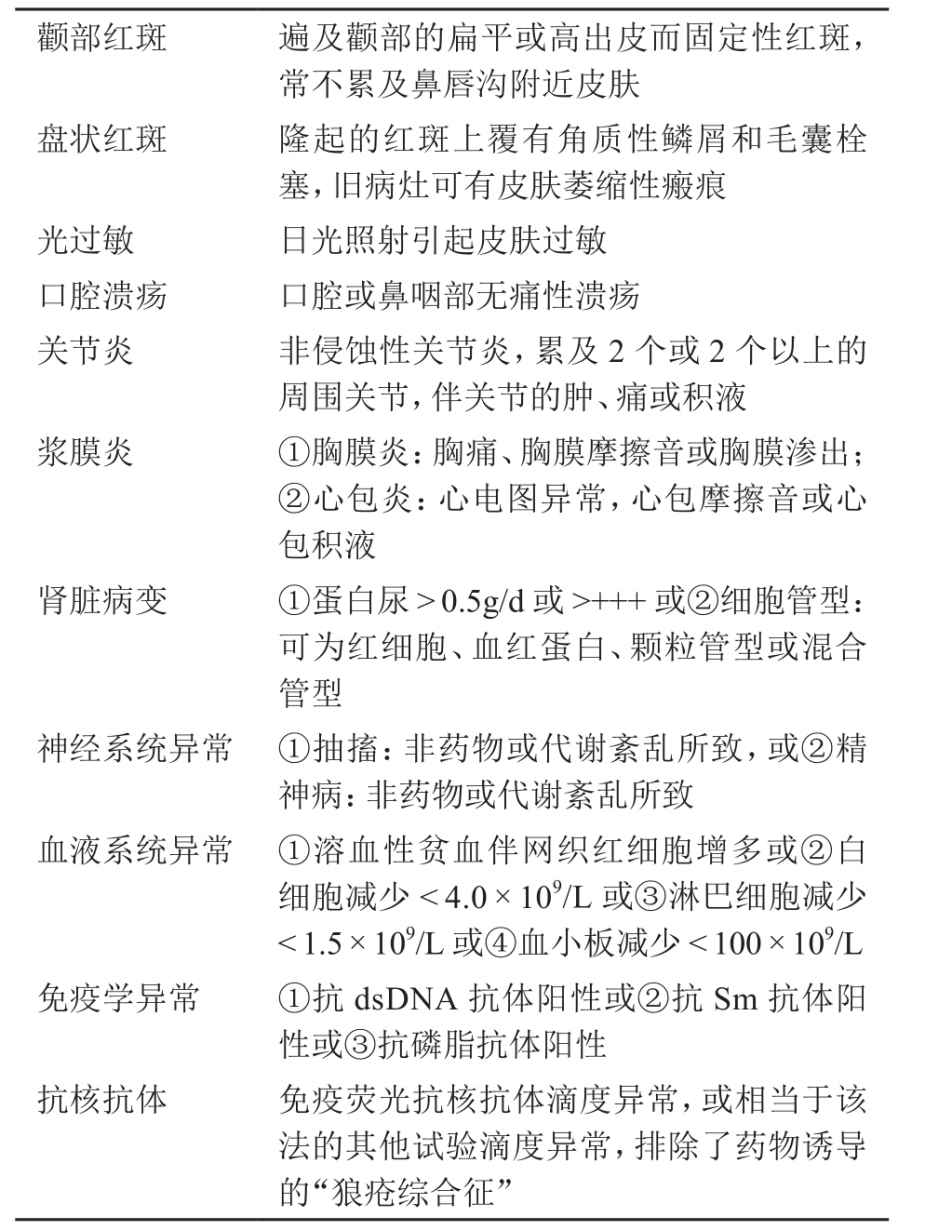
\includegraphics[width=3.30208in,height=4.39583in]{./images/Image00498.jpg}
\end{table}

\hypertarget{text00347.htmlux5cux23CHP14-1-2-3-3}{}
(三) 其他应注意的问题

1.有神经精神表现的 SLE患者
首先要明确该症状是SLE本身表现抑或并发症、治疗药物甚至并发神经精神疾病所致。进行脑脊液检查的主要目的是排除中枢神经系统感染,抗磷脂抗体与神经精神症状关系密切。CT对急性颅内出血临床诊断价值高,而在显示其他NPSLE病变如脑水肿等方面,MRI较CT有更高的敏感性,MRI之T2加权图像能显示NPSLE患者脑水肿发生的病理过程,比T1加权图像更加敏感。PET或SPECT检查可提供NPSLE患者脑血流、代谢功能有价值的信息。

2.肾活检
对狼疮肾炎的诊断、病理分期具重要意义,所提供信息非血清学检查及尿液分析所能替代,对患者的治疗,尤其是高危肾脏累及患者的治疗方案选择具指导意义,故对新发狼疮肾炎病例,主张常规进行肾穿刺活检。对治疗效果不佳及复发的患者,重复肾活检有助于了解患者病情恶化的原因,判断预后。对肾体积缩小、已经进展至终末期肾衰竭的SLE患者肾活检临床价值不大。

3.SLE患者胸膜炎、胸腔积液并非一定要进行胸腔穿刺术,考虑存在感染或其他原因时为穿刺指征。出现咳嗽、胸闷、呼吸困难等表现,要及时进行血常规、ESR、CRP、痰液病原学培养以及胸部X线平片、CT检查,必要时要进行支气管镜检查及动脉血气分析。狼疮性肺炎、肺出血、肺纤维化、卡氏肺囊虫感染等均表现为肺间质病变,影像学有诸多相似之处,一定要结合患者各项临床表现特点,综合分析,细心做出鉴别诊断。

4.每例急腹症患者都应尽快完善包括抗心磷脂抗体在内的血液学及生化检查
,症状隐袭出现者应尽早完善腹部超声、CT或磁共振等无创性检查。超声检查可发现增厚的肠壁,CT或磁共振可识别腹腔内脓肿、肿大的淋巴结、浆膜炎、增厚的肠壁、肠袢水肿及扩张、胰腺假囊肿以及肿大的肝、脾。腹部X线检查、腹腔穿刺术对诊断也能提供一定帮助。

5.SLE患者出现心悸、气促、水肿等表现要警惕心脏病变,应随时注意电解质、心肌酶学及心电图异常。并非每例心包积液均须心包穿刺,大量积液引起心包填塞、疑化脓性心包炎及其他不明原因心包积液者为穿刺指征。超声检查可显示SLE患者心包积液量及心包结构,SLE合并心肌炎时超声检查可显示心室扩大、射血分数下降、室壁活动异常等。食管超声检查检测心脏瓣膜病变具较高敏感性,同位素心肌灌注显像和冠状动脉造影有助于了解SLE冠状动脉粥样硬化及血管炎的严重程度。

\subsection{治疗}

SLE治疗原则是活动且病情重者,予以强有力的药物控制,病情缓解后,则接受维持性治疗。

\subsubsection{一般治疗}

包括:①患者教育是本病治疗的一个重要方面。②病情活动时注意休息,稳定后定期复查。妊娠、产褥期及手术患者应密切随访,以防复发或加重。③及早发现和治疗感染。④避免使用可能诱发SLE的药物,如避孕药等。⑤避免强阳光曝晒和紫外线照射。⑥女性SLE患者妊娠问题:无中枢神经系统、肾脏或其他脏器严重损害,病情处于缓解期达半年以上者,一般能安全地妊娠,并分娩出正常婴儿。非缓解期的SLE患者容易出现流产、早产和死胎,故应避孕。有习惯性流产病史或抗磷脂抗体阳性者,妊娠时应服低剂量阿司匹林(50mg/d)。

\subsubsection{糖皮质激素}

为治疗SLE主要的药物。对不甚严重病例,可先试用泼尼松0.5~1.0mg/(kg•d),晨起顿服,病情稳定后2周或疗程8周内,开始以每1~2周减10\%的速度缓慢减量,减至小于0.5mg/(kg•d)后,减量速度依病情适当调慢;维持量以小于10mg/d为宜。对有狼疮危象表现者须先用甲泼尼龙冲击疗法(0.5~1.0g/d静脉注射,连续3天),之后以口服大剂量泼尼松(>
30mg/d)维持,待病情控制以后逐渐减量。

\subsubsection{免疫抑制剂}

活动程度较严重的SLE,应同时给予大剂量激素和免疫抑制剂。加用免疫抑制剂有利于更好地控制SLE活动,减少SLE暴发,以及减少激素的需要量。狼疮肾炎用激素联合CTX治疗,会显著降低肾衰竭的发生。常用有环磷酰胺、硫唑嘌呤、环孢素、吗替麦考酚酯等。具体使用应因病情而异。

\paragraph{环磷酰胺(CTX)}

CTX冲击疗法,每次剂量0.5~1.0g/m\textsuperscript{2}
体表面积,加入生理盐水250ml中静滴,时间要>
1小时。除危重患者每2周冲击1次外,通常每4周冲击1次。冲击8次后,如病情明显好转,则改为每3月冲击1次,至活动静止后至少1年,可停止冲击。冲击疗法比口服疗效好。CTX口服剂量为1~2mg/(kg•d),分2次服。

\paragraph{硫唑嘌呤}

适用于中等度严重病例,脏器功能恶化缓慢者。常用量1~2mg/(kg•d)。常见副作用有胃肠道不适、肝损害和骨髓抑制。

\paragraph{环孢素}

每日5mg/kg,分2次口服,3个月。以后每月减少1mg/kg,至3mg/kg作维持治疗。主要副作用为肾、肝毒性,用药期间应予监测。

\paragraph{吗替麦考酚酯(MMF)}

其活性代谢物为霉酚酸酯。常用量1~2g/(kg•d),分2次口服。

\paragraph{抗疟药}

对皮疹、关节痛及轻型患者有效。羟氯喹200~400mg/d,分2次口服;氯喹250mg/d,1次口服。注意用药前和用药后每3~6个月进行眼科检查。

\subsubsection{静脉注射大剂量免疫球蛋白(IVIg)}

适用于某些病情严重或(和)并发全身性严重感染者,对重症血小板减少性紫癜有效。一般每日0.4g/kg静脉滴注,连续3~5天为1疗程。

\subsubsection{控制并发症与对症处理}

依病情选择治疗方案:

\paragraph{轻型}

以皮损和(或)关节痛为主,则可选用抗疟药,辅以非甾体类抗炎药。治疗无效应早用激素,泼尼松0.5mg/(kg•d)。

\paragraph{一般型}

有发热、皮损、关节痛及浆膜炎,并有轻度蛋白尿,宜用泼尼松,剂量0.5~1mg/(kg•d)。

\paragraph{狼疮肾炎(lupus nephritis,LN)}

依临床症状和病理分型选择治疗方案:①轻度肾脏损害:尿蛋白轻微(<
1g/d),血压、肾功能正常,病理表现为Ⅰ型或Ⅱ型者仅给予对症治疗。②局灶增生性LN:无临床和严重组织学病变活动者,可继续给予对症治疗或小剂量激素和(或)CTX;如有弥漫性节段性肾损害、大量蛋白尿、明显血尿和血肌酐升高者,治疗同弥漫增殖性LN。③膜性LN:表现为无症状蛋白尿和肾功能稳定者可给予对症治疗;肾病综合征者则需用大剂量泼尼松1mg/(kg•d)联合细胞毒药物治疗。④弥漫增殖性和严重局灶增殖性LN:活动性Ⅳ型LN伴近期内肾功能显著恶化者,可用甲泼尼龙15mg/(kg•d)冲击治疗,3天为1疗程,必要时2周后可重复1次,一般不超过3疗程。冲击后常规激素治疗,泼尼松1mg/(kg•d)×
8周,此后逐渐减量,直至5~10mg/d维持。常联合应用CTX。对大剂量激素及CTX无效或不能耐受者,可用环孢素或吗替麦考酚酯,常与中小剂量泼尼松合用。

\paragraph{NP-SLE}

甲泼尼龙冲击疗法和泼尼松每日1mg/kg,同时CTX冲击治疗,也可选用鞘内注射地塞米松10mg及甲氨蝶呤10mg,每周1次。有抽搐者同时给抗癫痫药、降颅内压等对症治疗。

\paragraph{溶血性贫血或(和)血小板减少}

予以甲泼尼龙冲击和泼尼松1mg(/kg•d),根据病情加用IVIg。

\paragraph{抗磷脂抗体综合征}

予以抗血小板药及华法林口服。

\paragraph{缓解期}

应使用不良反应最少的药物和用最小有效剂量,以达到抑制疾病复发的目的,如可每日晨服泼尼松5~10mg。

\subsubsection{血浆置换}

是短期的辅助治疗,可以迅速清除体内可溶性免疫复合物、抗基底膜抗体和其他免疫活性物质,为重症患者的治疗争取时间,不宜长期应用。临床用于治疗血栓性血小板减少性紫癜、肺出血及常规治疗不能控制的重症患者。

\subsubsection{人造血干细胞移植}

对于反复发作、难治性SLE可以采用异体自体干细胞移植治疗,其原理是利用大剂量免疫抑制剂摧毁自身免疫系统,并进行免疫重建,远期确切疗效还有待进一步研究。

\subsubsection{生物制剂}

目前用于临床试验治疗SLE的生物制剂主要有抗CD20单抗(利妥昔单抗,rituximab)和CTLA-4。

\subsubsection{其他几种特殊表现及处理}

\hypertarget{text00347.htmlux5cux23CHP14-1-3-9-1}{}
(一) 呼吸系统

\paragraph{急性狼疮肺炎}

发生率不高,但临床表现较重,发展快,死亡率高,见于病情活动期。表现为发热、咳嗽、少痰或无痰、呼吸困难、低氧血症。可有气促、咯血或胸痛。体检可发现双肺底细湿啰音,严重者可有中枢性发绀。影像学检查可见单侧或双侧较弥漫肺部浸润影,肺底为著。血WBC多正常,抗感染无效。需注意与急性肺部感染鉴别。后者常发生在应用激素及免疫抑制剂治疗过程中,患者常高热、进行性呼吸困难、短期内发展为“白肺”,起病前多有前驱受凉感冒病史。

处理:①呼吸支持治疗:多数患者需要氧疗,严重低氧血症需机械通气。②糖皮质激素:常需大剂量糖皮质激素,必要时可甲泼尼龙冲击治疗。③免疫抑制剂:对糖皮质激素反应差者可应用免疫抑制剂如硫唑嘌呤、环磷酰胺。

\paragraph{急性肺泡出血}

少见,但死亡率极高,多同时存在其他系统损害、高滴度ds-DNA抗体及低补体血症。临床表现与急性狼疮肺炎类似,常突然出现发热、呼吸困难、咳嗽、痰中带血,少数情况下出现咯血。可数小时到数天内出现气促、低氧血症、心动过速、急性呼吸窘迫。突然血红蛋白及血细胞比容下降常有提示作用。影像学多为双肺弥漫性浸润渗出影。由于咯血并非每个患者均出现,故肺出血常被贻误。若患者出现血细胞比容及血红蛋白迅速下降、弥漫性肺部浸润,应当警惕肺出血。支气管肺泡灌洗液多为血性。需注意与急性左心衰竭、肺部感染、非心源性肺水肿相互鉴别。

处理:首选大剂量糖皮质激素,必要时可甲泼尼龙冲击治疗。免疫抑制剂可根据情况选用。上述治疗无效者可行血浆置换。其他措施包括氧疗、机械通气等对症支持治疗。

\paragraph{肺萎陷综合征(shrinking lung syndrome)}

为SLE罕见并发症,表现为不明原因呼吸困难,常无全身性炎症表现。胸部X线显示肺容积减少、患侧膈肌抬高、活动度差、基底肺不张,但无膈肌矛盾运动,常无肺间质及肺血管病变。肺功能检查提示限制性通气障碍。发病机制可能与膈肌无力、胸膜炎症有关。一般认为本病进展缓慢,预后良好,但亦有导致呼吸衰竭需要机械通气的报道。处理:首选糖皮质激素,常用泼尼松30~60mg/d。可合用β-肾上腺素受体激动剂及茶碱。难治性病例可选用免疫抑制剂如甲氨蝶呤、环磷酰胺等。

\hypertarget{text00347.htmlux5cux23CHP14-1-3-9-2}{}
(二) 恶性抗磷脂综合征

恶性抗磷脂综合征(catastrophic anti-phospholipid
syndrome,CAPS)指抗磷脂综合征短期内出现多器官衰竭的疾病形式。临床特点包括:短期内出现多器官损害;多部位小血管阻塞证据;高滴度抗磷脂抗体;60\%病例发病前有前驱事件(主要是感染,其他包括:创伤、停用抗凝药物、妊娠、合并肿瘤等)。CAPS临床表现取决于2个因素:血栓事件所及器官和血栓程度;全身炎症反应(SIRS)的临床表现。

CAPS与经典APS相比具有以下特点:①可有不寻常的器官累及,如卵巢、子宫、睾丸梗死;②肺部并发症发生率高,如ARDS及弥漫性肺泡出血;③腹痛常见,与腹腔内血栓导致肠、胆囊、胰腺、肾上腺、脾脏血管栓塞有关;④可因SIRS导致意识丧失;⑤1/5患者可出现DIC;⑥严重的血小板减少可致出血(尤其颅内出血);⑦妊娠者HELLP综合征发生率高;⑧预后差。

腹腔内血栓事件最常见,肾脏、肾上腺、脾脏、肠道、肠系膜及胰腺血管最常受侵,患者常主诉腹痛或腹部不适。肺部并发症其次,与ARDS或肺栓塞有关,尚可出现肺出血、微血栓、肺水肿等,常主诉呼吸困难。皮肤表现有网状青斑、紫癜、皮肤坏死。中枢表现常见为:梗死、脑病、癫痫、中枢静脉梗阻。心脏事件发生率为53\%,瓣膜病最为常见(主要是二尖瓣及主动脉瓣)。少数亦可出现心肌梗死。其他器官受累包括:睾丸/卵巢梗死、前列腺坏死、无结石性胆囊炎、骨髓梗死、食管破裂、巨大消化道溃疡、结肠溃疡、血栓性胰腺炎、肾上腺梗死等。

实验室检查:60\%有血小板减少,1/3可有溶血,但碎裂红细胞较少,1/5有DIC。IgG型抗磷脂抗体常见,IgM型抗磷脂抗体则相对较少。

CAPS诊断标准:①3个或以上的器官、系统血栓事件;②临床表现常于1周内相继出现;③组织病理学表明至少1个器官或组织存在小血管阻塞;④抗磷脂抗体阳性。符合以上4条为肯定CAPS;很可能CAPS为:①符合4条,但仅2个器官或系统受累;②符合4条但由于严重血栓事件患者死亡且6周之前未曾查过抗磷脂抗体;③符合①②④条;④符合①③④条。

处理:①一线治疗:抗凝治疗,首选静脉应用肝素(1500U/h)连用7~10天,之后改为口服抗凝剂,使INR维持在2~3。糖皮质激素用于控制SLE病情活动,多用泼尼松1~2mg(/kg•d),尤其适用于合并ARDS及急性肺泡出血患者。②二线治疗:静脉应用丙种球蛋白,用量为0.4g(/kg•d),连用4~5天。对严重血小板减少患者尤为有效。与血浆置换联用可提高疗效。③三线治疗:可选择免疫抑制剂如环磷酰胺,理论上能够预防血浆置换后抗磷脂抗体反跳。治疗反应不佳的严重血小板减少可试用利妥昔单抗。

\hypertarget{text00347.htmlux5cux23CHP14-1-3-9-3}{}
(三) 巨噬细胞活化综合征

巨噬细胞活化综合征(macrophage activation
syndrome,MAS)是与自身免疫疾病相关的嗜血细胞综合征的特殊类型。常突然急性起病,进展迅速,若不能及时诊治,死亡率极高。临床表现为高热、肝脾淋巴结肿大、外周血细胞减少、肝功能异常、凝血障碍、高甘油三酯血症、高铁蛋白血症。此外,血液及脑脊液中NK细胞活性下降和可溶性CD25(sCD25,是IL-2可溶性受体)水平升高。组织病理学可见大量淋巴细胞、成熟巨噬细胞和组织细胞浸润脾脏、淋巴结、骨髓、肝脏及脑脊液。有时早期患者骨髓检查可能正常,故反复骨髓检查有利于诊断。SLE发生MAS常与高度活动的病情或继发感染有关。因此应当注意鉴别SLE并MAS的诱因。目前尚未有SLE合并MAS统一诊断标准。当出现原发病不好解释的多系统受累的危急情况时应当想到MAS的可能;当患者出现持续性发热、不明原因的全血细胞减少及凝血异常、高甘油三酯血症、迅速出现的肝脾淋巴结肿大应当警惕MAS。

处理:SLE并MAS治疗原则为:积极治疗原发病,控制炎症瀑布。

\hypertarget{text00347.htmlux5cux23CHP14-1-3-9-3-1}{}
(1) 病因治疗:

鉴别SLE病情活动导致MAS抑或感染诱发MAS非常重要。若是SLE病情活动未控制,则当应用大剂量糖皮质激素甚至静脉冲击治疗,若为感染诱发,则当积极控制潜在的感染。

\hypertarget{text00347.htmlux5cux23CHP14-1-3-9-3-2}{}
(2) 免疫抑制剂:

可应用环磷酰胺、环孢素、长春新碱等。亦可应用VP-16。

\hypertarget{text00347.htmlux5cux23CHP14-1-3-9-3-3}{}
(3) 丙种球蛋白:

对于难以鉴别感染或原发病活动的患者可应用。

\hypertarget{text00347.htmlux5cux23CHP14-1-3-9-3-4}{}
(4) 生物制剂:

有报道TNF-α拮抗剂、IL-6拮抗剂有助于阻断细胞因子大量释放所致的炎症瀑布。抗胸腺球细胞蛋白联合糖皮质激素和环孢素可诱导缓解。

\hypertarget{text00347.htmlux5cux23CHP14-1-3-9-3-5}{}
(5) 其他:

对治疗反应差的难治性病例可考虑造血干细胞移植。

\hypertarget{text00347.htmlux5cux23CHP14-1-3-9-4}{}
(四) 妊娠相关问题

妊娠使
SLE病情活动风险增加2~3倍,大多数活动度轻微增加,只有15\%~30\%活动度高。妊娠期常见的病情活动表现是皮肤病变、关节炎、血液系统损害及狼疮肾炎。妊娠期病情活动的预测因子有:孕前6月内病情活动、孕前1年内有多次复发活动、停用羟氯喹。

\paragraph{鉴别先兆子痫和 SLE复发活动}

二者均可出现蛋白尿、高血压、下肢水肿及多系统损害,但二者处理却截然不同:前者需立即终止妊娠,后者则需增强免疫抑制力度。表\ref{tab125-2}\footnote{备注:sFlt-1,soluble FMS-like tyrosine
kinase-1,可溶性FMS样酪氨酸激酶-1;PlGF,placental growth
factor,胎盘生长因子}中各项指标有助于二者鉴别。但应当注意,SLE尤其是狼疮肾炎复发活动可与先兆子痫同时存在。

\paragraph{妊娠期血压控制}

合并高血压的SLE患者妊娠前必须停用ACEI和ARB,因其可导致胎儿心脏和脑发育异常。但这将导致尿蛋白量增加、血压难以控制。但幸运的是妊娠早期和中期血压有下降趋势。若是患者一直服用噻嗪类利尿剂,则不必停用。应避免应用袢利尿剂,因其可导致胎盘血流量不足。非孕SLE患者降压目标为120/80mmHg,但妊娠期SLE降压目标为140/90mmHg,以免导致胎盘血流量下降。降压药可选用拉贝洛尔。

\begin{table}[htbp]
\centering
\caption{先兆子痫和 SLE复发活动的鉴别}
\label{tab125-2}
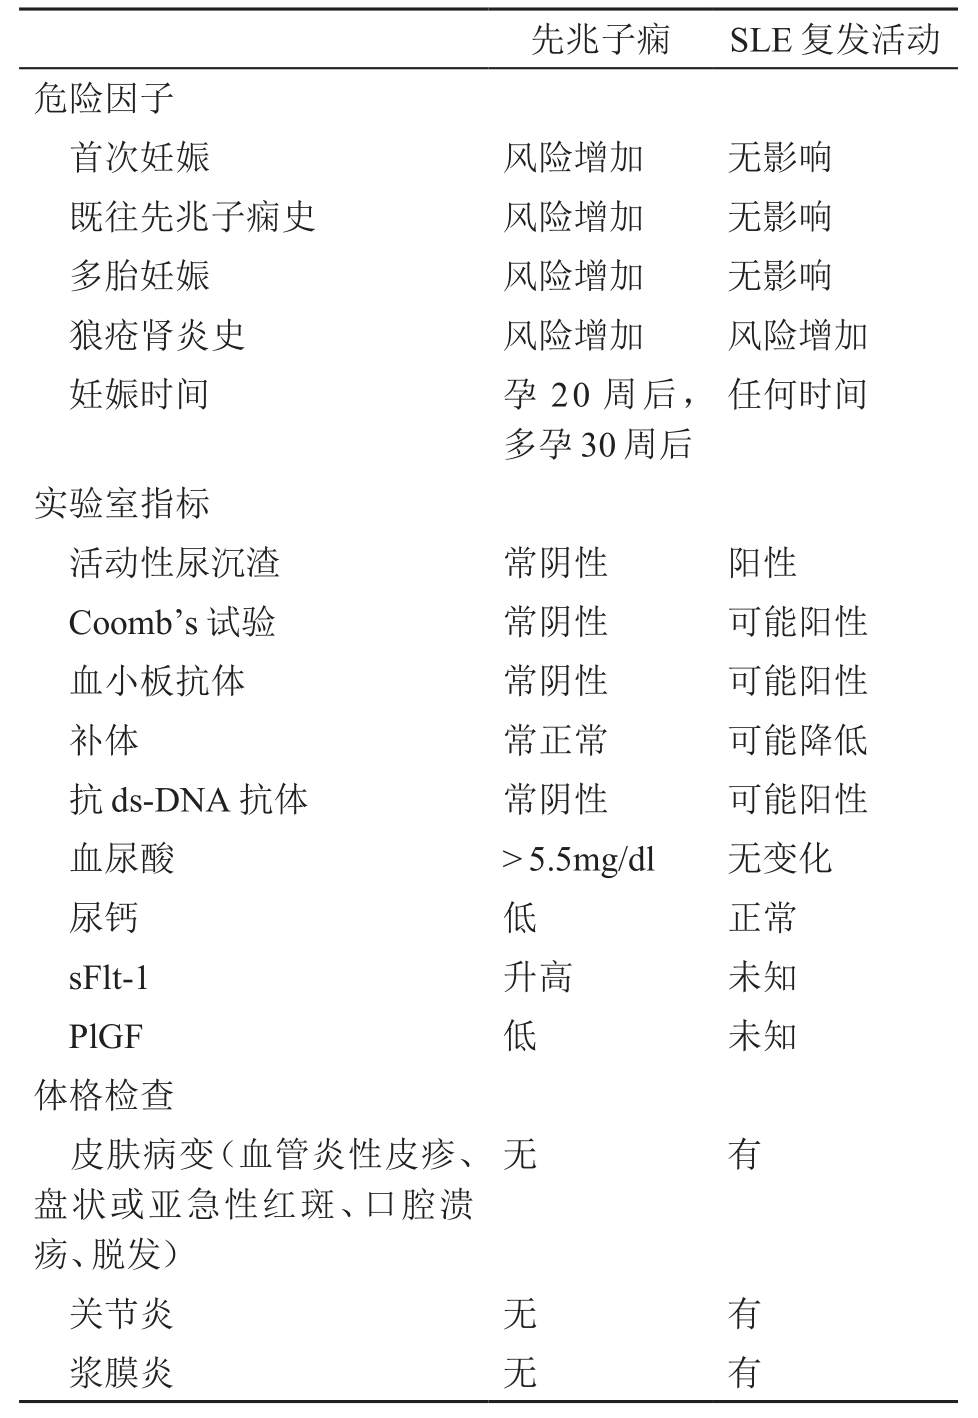
\includegraphics[width=3.25in,height=4.71875in]{./images/Image00499.jpg}
\end{table}


\paragraph{SLE妊娠期病情活动的控制}

①无病情活动者不需要特殊处理,每4~6周随访1次。②轻度活动者仅需低剂量泼尼松维持(≤20mg/d)。③中度活动者需较大剂量糖皮质激素维持,甚至冲击剂量。其他选择包括静脉丙种球蛋白冲击。对控制血液系统病变及狼疮肾炎有效。④对于病情难以控制,短期内又不能期待生产者应考虑终止妊娠。

\paragraph{新生儿狼疮综合征(neonatal lupus syndrome)}

新生儿狼疮综合征是一种被动传输的自身免疫病,其发生与母体内的抗SSA/Ro和(或)抗SSB/La抗体有关,可累及多个器官,包括心脏、皮肤、肝脏和血液。

\hypertarget{text00347.htmlux5cux23CHP14-1-3-9-4-4-1}{}
(1) 先天性房室传导阻滞(CAVB):

被定义为出生前、出生时或出生后0~27天内诊断的房室传导阻滞(AVB)。抗SSA/Ro和(或)抗SSB/La抗体阳性的母亲其胎儿发生CAVB的风险为2\%,而生产过CAVB婴儿的母亲再次妊娠发生同样情况的风险则增加至15\%。CAVB常发生于妊娠的16~24周,若不能及时发现和治疗,将逐渐由Ⅰ度AVB发展为不可逆的Ⅲ度AVB。因此建议所有患有结缔组织病的女性妊娠前应当筛查抗SSA/Ro和抗SSB/La抗体,若阳性则应视为高危患者,建议妊娠16~26周每周检查一次胎儿心脏彩超,妊娠26~32周每2周检查一次胎儿心脏彩超,以期早期发现PR间期延长。有学者认为胎儿心电图(FKCG)比胎儿彩超更加敏感,能够早期发现Ⅰ度AVB。

处理:一旦发现CAVB,应当立即开始治疗。①对于一度、二度AVB及二度、三度交替的AVB,建议母亲口服地塞米松4mg/d直至分娩,若持续6周仍无改善或进展至三度AVB则逐渐减量至停用。②对于病程<
2周的三度AVB,建议母亲口服地塞米松4mg/d,共6周。若转变为二度AVB或改善更好,则继续服用直至分娩,然后逐渐减量至停用。若无好转,则应逐渐停用。③对于病程>
2周的三度AVB,不应再积极治疗,而应每周检查胎儿心脏彩超。④AVB同时合并心肌炎、充血性心衰或水肿,应口服地塞米松4mg/d直至病情改善。⑤若胎儿有严重水肿可口服地塞米松4mg/d,若胎儿心率<
50~55次/分,亦可考虑使用β受体激动剂以提高心率。如口服特布他林2.5~7.5mg,4~6小时1次,最大量30mg/d;口服沙丁胺醇10mg,8小时1次,最大量40mg/d,一般能够增加心室率5~10次/分。β受体激动剂副作用包括颤抖、心悸和出汗,一般可耐受并逐渐改善甚至消失。对于合并糖尿病、高血压、甲状腺功能亢进症及既往有癫痫或快速性心律失常的母亲应避免应用β受体激动剂。若胎肺成熟应尽早终止妊娠。有新生儿立即行积液引流、应用异丙肾上腺素及临时起搏抢救成功的报道。⑥此外尚可考虑静脉应用免疫球蛋白治疗AVB。

\hypertarget{text00347.htmlux5cux23CHP14-1-3-9-4-4-2}{}
(2) 其他表现:

包括狼疮样皮损、一过性血液系统改变等,常产后6~8周随抗体逐渐清除而慢慢消失。皮损可局部外用非氟化糖皮质激素。

\hypertarget{text00347.htmlux5cux23CHP14-1-3-9-5}{}
(五) SLE与应激

SLE患者长期服用糖皮质激素将导致下丘脑-垂体-肾上腺(HPA)轴抑制,当遇到应激时不能够分泌足够的促肾上腺皮质激素(ACTH)和可的松,因此在应激状态下需要外源性补充糖皮质激素(即应激剂量“stress
dose”steroids)以提高患者应激能力。此时常需要回答2个问题:①患者的糖皮质激素剂量和服用时间是否已经引起HPA轴抑制?②若HPA轴被抑制,应当补充多少剂量糖皮质激素?

HPA轴是否被抑制与年龄、性别、用药时间、累积剂量并非绝对相关,且不同个体之间变异较大。但是目前已知每日晨服泼尼松<
5mg持续任何时间、隔日晨起口服短效糖皮质激素任何剂量持续任何时间、任何剂量糖皮质激素服用时间不超过3周都不会引起HPA轴的明显抑制。但是若服用每日剂量超过20mg泼尼松或同等剂量的糖皮质激素超过3周的患者、已经有明显Cushing面容的患者很可能有HPA轴的抑制。糖皮质激素停用后HPA轴的抑制将持续多长时间目前尚无定论。既往研究提示糖皮质激素停用后1年仍可检测到HPA轴的抑制。因此建议若有HPA轴抑制,1年内手术均应补充糖皮质激素。

对于正在应用中等剂量糖皮质激素或不能提供用药史(包括剂量、用药时间、如何减量等信息)的患者,若术前时间充裕可用低剂量(1g)ACTH刺激试验检测HPA轴状态。围术期糖皮质激素替代治疗方法详见表\ref{tab125-3}。

\hypertarget{text00347.htmlux5cux23CHP14-1-3-9-6}{}
(六) SLE与感染

SLE患者感染高危因素包括:先天性低补体血症、SLE病情活动、服用大剂量糖皮质激素、同时应用免疫抑制剂、技术操作(如:血浆置换者同时应用环磷酰胺感染风险明显增加,接受腹膜透析的SLE患者腹膜炎、导管相关感染风险增加)。感染是SLE患者死亡的最主要原因。

\begin{table}[htbp]
\centering
\caption{围术期糖皮质激素替代治疗方法}
\label{tab125-3}
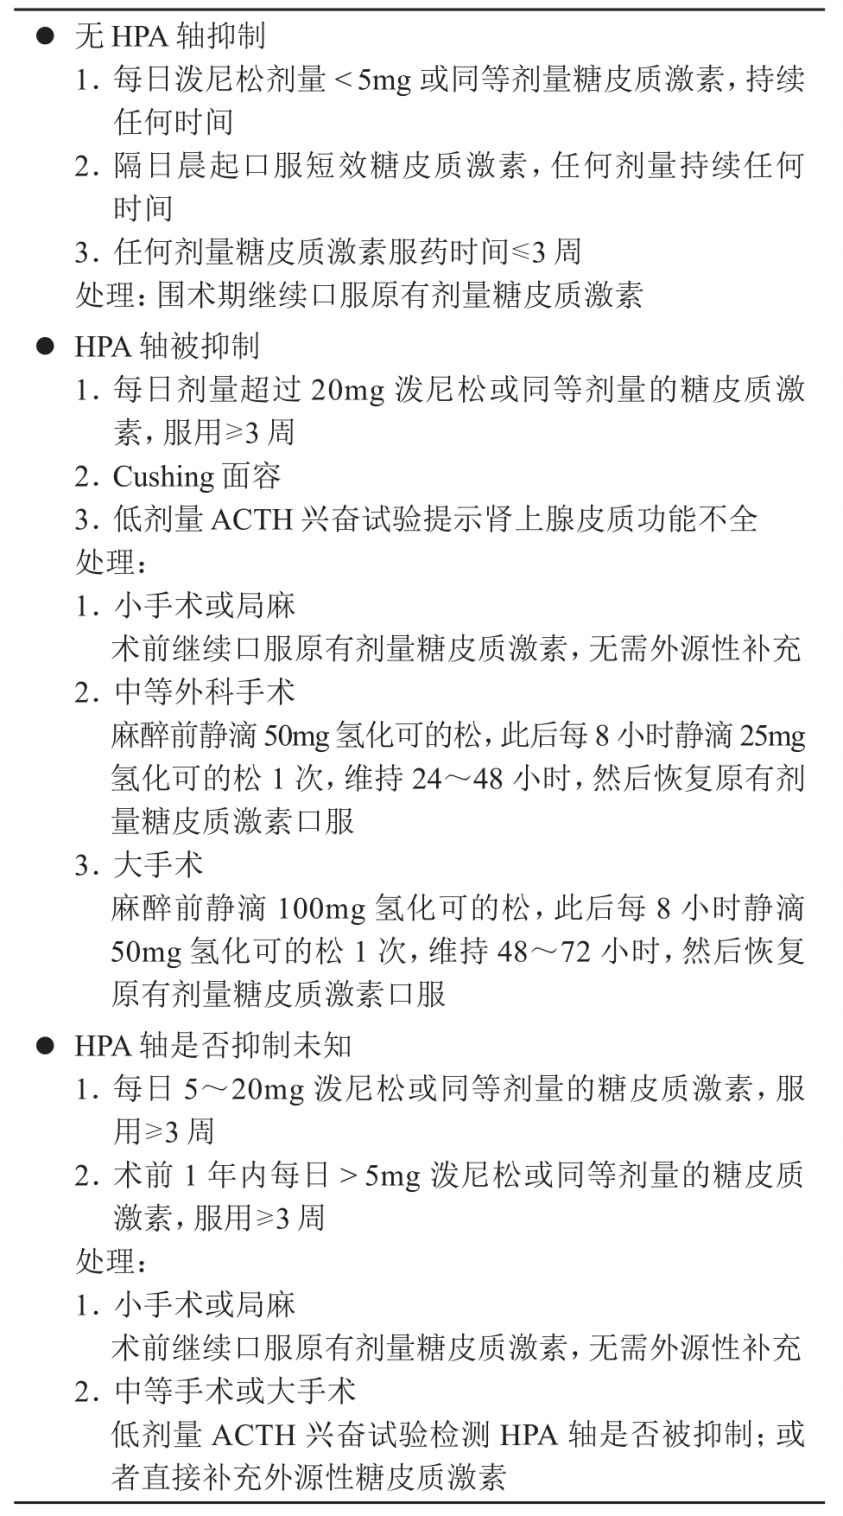
\includegraphics[width=3.25in,height=5.83333in]{./images/Image00500.jpg}
\end{table}

SLE患者感染的部位常见为:呼吸道(包括肺部)、泌尿道、肠道、中枢神经系统、血液、皮肤等。病原体有细菌、病毒、真菌及寄生虫,其中细菌感染最为常见,占SLE所有感染的90\%。革兰阳性球菌常见金黄色葡萄球菌(引起皮肤、骨和关节感染,少见情况可引起败血症、肺炎、导管相关感染)、肺炎球菌(引起肺炎,甚至败血症、颅内感染)。革兰阴性杆菌常为大肠杆菌、克雷伯杆菌、假单胞菌等,常引起泌尿道、下呼吸道感染,甚至败血症。

活动期SLE尚可出现沙门菌感染,包括猪霍乱沙门菌、肠炎沙门菌、鼠伤寒沙门菌等。沙门菌感染在SLE患者有较高的病死率,常发生于SLE活动期及正接受糖皮质激素、免疫抑制剂治疗的患者。可表现为菌血症、胃肠炎、关节炎、肺炎、泌尿道感染、软组织脓肿、骨髓炎、脑膜炎等肠外病变,中毒症状不明显,15\%~20\%的患者可不发热,典型的伤寒症状少见。治疗不彻底常可复发。

其他机会性细菌感染有诺卡菌病、分枝杆菌感染(主要是结核分枝杆菌)。诺卡菌感染临床特点为脏器单发或多发脓肿形成,常见于肺、脑、皮下等部位。努卡菌肺部感染表现为肺内单个或多个结节状阴影,常形成空洞,伴胸壁扩张。SLE患者易发生结核分枝杆菌感染,肺外结核及粟粒样肺结核常见,病死率高。除疾病本身外,使用糖皮质激素、疫区居住史、既往结核病史或PPD阳性均为结核感染的危险因素。硬结直径在0.5cm以上者即可认为阳性。

病毒感染最常见为带状疱疹病毒,常发生于既往有狼疮肾炎、溶血性贫血、血小板减少及应用环磷酰胺的SLE患者,多为局部感染,但也有全身播散合并细菌感染的情况,多见于应用大剂量糖皮质激素(泼尼松≥60mg/d)或免疫抑制的SLE患者。巨细胞病毒亦较常见,发生于应用大剂量糖皮质激素、环磷酰胺或血浆置换的SLE患者,常引起致命的肺炎和脑炎。

真菌感染最常见为曲霉菌、卡氏肺孢子菌及念珠菌感染。前两者常导致严重的肺部感染,后者病变范围广泛,卡氏肺囊虫性肺炎几乎总发生于正接受免疫抑制剂治疗的患者,往往发病急,胸闷、呼吸困难症状明显,胸片或肺部CT检查可发现肺部间质性肺纤维化改变。留置插管及应用广谱抗生素者应注意念珠菌感染,可导致口腔及食管黏膜、泌尿生殖道感染,但播散性念珠菌病较少见,但一旦发生常致命。新型隐球菌性脑膜炎常潜隐发病,神经系统表现无特征性,易被误诊为NPSLE。

处理要点:

1.鉴别是感染还是 SLE病情活动
SLE合并感染最常见的表现是发热。每一例SLE患者出现发热必须注意感染的可能,尤其是正在接受糖皮质激素和免疫抑制剂治疗者。合并呼吸道、泌尿生殖道、肠道感染者常有相应症状和体征,不难鉴别。但有时临床鉴别二者相当困难,以下可作参考:①原本病情稳定者突然发热,多考虑合并感染。②发热伴有寒战多为感染。③血沉和CRP明显升高者多提示感染。SLE合并感染性发热时,足量糖皮质激素亦不能使体温维持在正常水平。详细询问病史、体格检查是正确诊断的前提。对于鉴别困难而又高度怀疑合并感染者常需全面寻找感染灶,尤其注意常易忽视的部位(如皮肤、腹腔、盆腔、腹膜后、肛周、颅内等),积极、反复进行体液及排泄物(包括血液、骨髓、痰液、尿液、粪便)等的培养,行CT、MRI等影像学检查等。T-Spot是目前筛查隐匿性结核感染的有力工具,但其阴性并不能排除结核感染。

2.一旦明确
SLE合并感染,应当立即进行抗感染治疗,停用所有免疫抑制剂。长期应用糖皮质激素者此时不能停用,以免降低机体应激能力,而应当根据患者病情考虑酌情减量、维持原量还是适当加量。对于合并感染且病情活动者或病情活动与感染不易鉴别者,丙种球蛋白冲击治疗不失为一举两得的良策。

\protect\hypertarget{text00348.html}{}{}

\chapter{结节性多动脉炎}

“多动脉炎”一词是一个模糊的概念,通常是指多种血管炎,但结节性多动脉炎(polyarteritis
nodosa,PAN)的定义随着时间的推移发生了巨大的变化,以往的“PAN合并类风湿关节炎”现在已经被命名为类风湿性血管炎。1994年在(Chapel
Hill Consensus
Conference,CHCC)有关系统性血管炎命名的会议上将PAN已经专用于描述中小肌性动脉坏死性血管炎(medium
vessel
vasculitis,MVV),受累动脉直径在50~150μm。抗中性粒细胞胞浆抗体(ANCA)通常为阴性,这种小动脉不包括细动脉、小静脉及毛细血管并且与肾小球血管无关。

\subsection{病因与发病机制}

\subsubsection{病因}

结节性多动脉炎的发病原因尚未十分明了,一般认为与下列因素有关:

\paragraph{免疫复合物}

自1905年Pirquet等观察到给人体注射马白喉抗毒素后引起皮疹、关节炎、动脉炎和肾炎以来,人们相继相信免疫复合物对结节性多动脉炎的影响。近年Dixon等将牛血白蛋白静脉注入家兔,引起动脉炎,所以,认为异种血清引起的免疫复合物是引发本病的可能病因。

\paragraph{药物}

1942年Rich报道了磺胺类药物引起结节性多动脉炎病例。此后,药物诱发本病的问题引起人们的广泛关注。现已肯定了某些药物是该病发病的原发病因,如青霉素、氯霉素、四环素、磺胺类、硫脲嘧啶等,麻醉剂和兴奋剂亦可诱发本病。

\paragraph{感染}

细菌和病毒感染是结节性多动脉炎的重要发病原因,其中病毒可能是重要的致病因素,30\%~50\%的结节性多动脉炎患者和乙型肝炎病毒持续感染密切相关,并从本病的病变部位证实了有乙肝抗原。其他的病毒有人类免疫缺陷病毒、巨细胞病毒、甲型肝炎病毒、丙型肝炎病毒、I型人类T细胞白血病病毒、副病毒等。所以,认为结节性多动脉炎可能是病毒作为抗原的免疫复合物病。某些细菌特别是溶血性链球菌引起的变态反应可以导致多动脉炎或引起多动脉炎类似的病变。真菌,寄生虫同样也可引起相似的结节性动脉炎的表现。

\subsubsection{发病机制}

与PAN的病因一样,其发病机制也不十分明确。1925
年Gruber最先提出变态反应学说,之后有人强调高血压在发病中的作用,认为血管炎尤其是坏死性血管炎的发生与血流动态有密切关系,而遗传学研究发现,本病有先天性C\textsubscript{2}
缺乏和α\textsubscript{1} -抗胰蛋白酶缺乏。

病毒感染可以导致内皮细胞功能的变化,使内皮细胞表达IgG的Fc受体、C3b受体并和主要组织相容性复合体Ⅱ类分子(MHCⅡ)结合进一步产生IL-1,导致血管内皮细胞的损伤和功能的紊乱。损伤的内皮细胞可释放血小板活化因子(PAF)、IL-1、血管内皮生长因子(VEGF)、肿瘤坏死因子(TNF),由于细胞因子的相互作用,使得正常的内皮细胞破坏,成为凝血过程的启动环节,使内皮细胞对中性粒细胞、单核细胞、淋巴细胞黏附性增强,受损的内皮细胞进一步释放多种细胞因子,产生炎症,形成免疫反应灶。干扰素和TNF能诱导内皮细胞表达MHCI类分子,而T细胞可以识别内皮细胞表达的MHCI类分子,继而杀伤内皮细胞,加重内皮细胞的损伤。

药物、疫苗、细菌感染、病毒感染引起的变态反应,形成可溶性循环免疫复合物沉着于血管壁,造成血管壁通透性增强,补体被激活,免疫活性细胞浸润,导致血管炎性病变或发生坏死,是结节性多动脉炎的重要发病机制之一。

PAN的特征性病理改变,主要是中小肌性动脉的全层坏死性血管炎,病变呈现局灶性,阶段性,好发于动脉的分叉部位和血管进入脏器之处。病变常常从中动脉壁中层开始,再扩展到内膜和外膜,常可破坏内弹力层。PAN病变可累及任何脏器的动脉,但较少累及肺和脾动脉。病理上分为初期(变性期)、急性炎症期、好转期(肉芽肿形成期或慢性期)和治愈期(瘢痕期)等4期改变,各期病变可同时存在。肾脏、肝脏、心脏及胃肠道受累最常见。

\subsection{诊断}

\subsubsection{临床表现特点}

PAN的受累表现可以分为局限型和系统型:

\paragraph{系统型}

由于病变分布不规则,临床上可以出现不同区域血管的坏死及炎症,从而出现多种临床表现。见表\ref{tab126-1}。

\paragraph{局限型}

以局限于皮肤者多见,主要累及真皮、皮下小动脉,发生坏死性炎症,临床以皮下结节、网状青斑和肌痛为主要症状,亦可累及肌肉和周围神经。皮肤型多动脉炎累及皮下组织的小动脉,通常不损害内脏动脉,呈慢性局限性的过程,病程长,预后好。

\subsubsection{辅助检查}

PAN的实验室检查不具有特异性。

\begin{table}[htbp]
\centering
\caption{系统型结节性多动脉炎的临床表现}
\label{tab126-1}
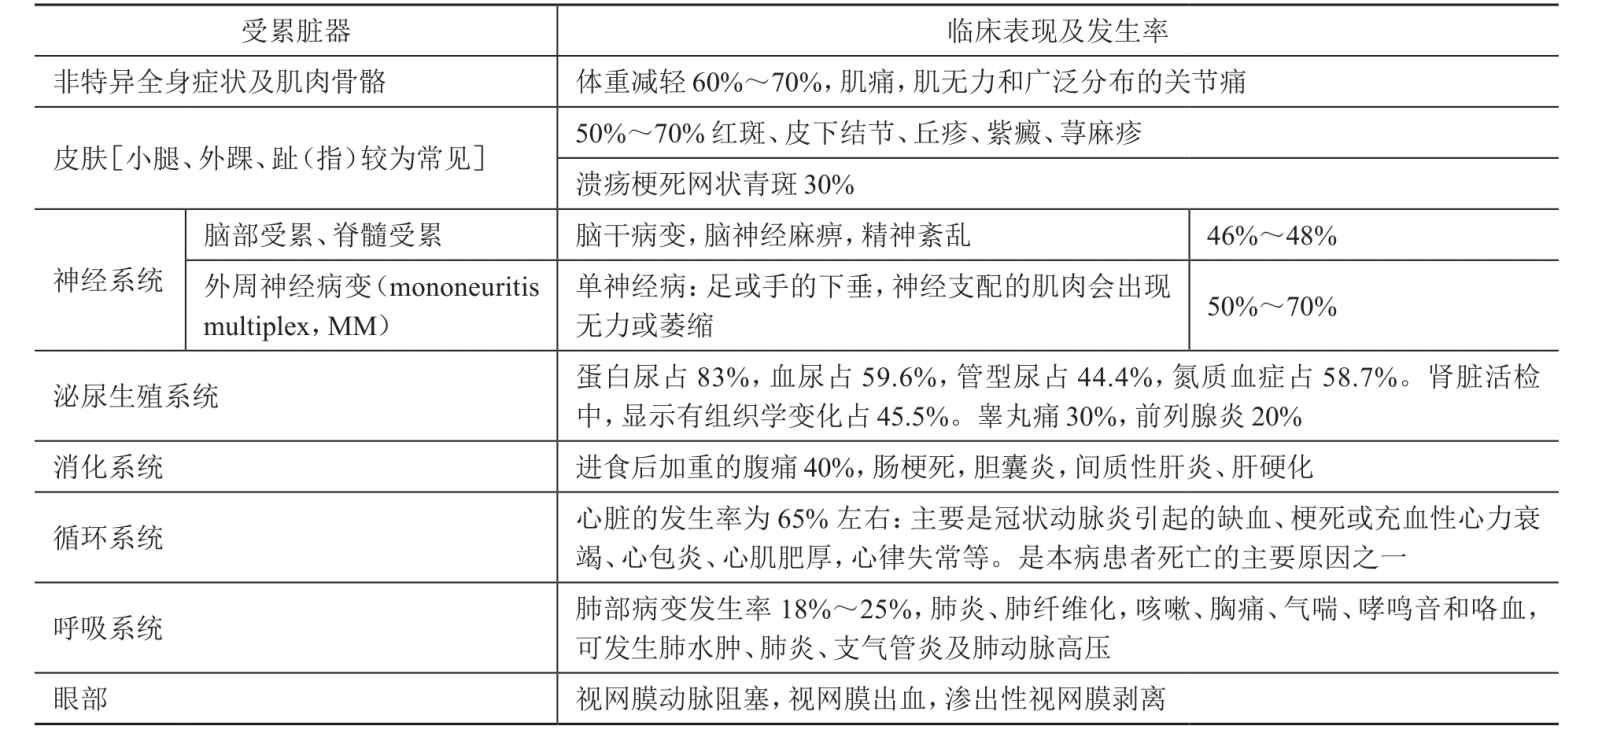
\includegraphics[width=6.78125in,height=3.15625in]{./images/Image00501.jpg}
\end{table}

\paragraph{一般检查}

血液学检查可提示贫血,白细胞增多,血小板增多;尿常规检查提示:镜下血尿、蛋白尿、管型尿等变化,血沉增快,CRP升高,血清白蛋白减少,肝肾功能异常。

\paragraph{免疫学检测}

部分患者可以出现总补体水平及补体C3,C4下降,部分患者可以出现类风湿因子阳性及低滴度的抗核抗体、冷球蛋白、抗核周型中性粒细胞胞浆抗体(p-ANCA)。抗髓过氧化物酶(抗MPO)抗体对结节性多动脉炎的诊断价值日益受到重视。研究表明抗MPO抗体为结节性多动脉炎尤其是合并肺、肾损害者的敏感指标,抗MPO抗体和疾病活动性相关,可作为疾病活动期的指标。

\paragraph{影像学检查}

包括普通胸腹部X线检查及内脏动脉造影。动脉血管造影是确诊PNA的重要手段之一。动脉瘤最常发生在肾、肝动脉,也见于肠系膜,脑、脾、肺、肋间、膈下、胃上和十二指肠动脉。中小动脉囊性或纺锤形的微小动脉瘤,节段性动脉狭窄和动脉变细(剪枝样中断),肠系膜动脉造影可以作为PAN患者严重腹痛时选择的检查。

\paragraph{活体组织检查}

活检获得病理学证据是PAN重要的诊断依据之一。活检要遵循以下原则:取材方便的部位:皮肤、肌肉、睾丸、神经;肌电图显示有神经受累时,活检的神经应在神经横截面有足够的小动脉。国外常用的活检部位为腓肠神经;如果其他部位不能提供诊断所需的材料,对有肾炎者作肾脏活检,对严重肝功能异常者作肝脏活检是可取的。

\paragraph{其他辅助检查}

心电图和超声心动图,腹部B超有助于发现肝胆胰肾受累的情况,内镜可以检查胃肠受累的情况,肌电图检查可以发现神经及肌肉的受累,出现中枢神经系统症状时,还应进行头颅CT及MRI的检查。

\subsubsection{诊断注意事项}

结节性多动脉炎为全身性疾病,具备典型的临床表现诊断并不困难。然而早期临床表现多样,缺乏特异性,不易诊断,而治疗是否及时直接影响预后。当有迅速发展的高血压伴有不明原因发热、腹痛、肾功能衰竭时,或当疑似肾炎或心脏病患者伴有嗜酸性粒细胞增多或不能解释的症状和关节痛、肌肉压痛与肌无力、皮下结节、皮肤紫癜、腹部或四肢疼痛、或迅速发展的高血压时,可拟诊结节性多动脉炎。特别是当其他发热,多脏器损伤的原因已被排除时,临床与实验室检查结果通常可提示诊断。全身性疾病伴两侧对称或不对称地累及主要神经干(如桡神经、腓神经、坐骨神经)的周围神经炎(通常为多发性,即多发性单神经炎)提示为结节性多动脉炎,原来健康的中年男性发生上述临床表现者亦提示结节性多动脉炎。

由于缺乏PNA的统一诊断标准,目前沿用的为1990年美国风湿病学会关于PNA的分类标准(表\ref{tab126-2})。在10项中有3项阳性者即可诊断为PNA。但在诊断时应排除其他结缔组织病并发的血管炎。

由于本病累及范围较广,临床表现特异性差,故必须与多种疾病鉴别。

其他原发和继发的血管炎病:各种系统性血管炎的临床表现既有特征性,又有部分重叠,故应从发病年龄、伴随疾病、血管类型、分布和病理特点等几方面加以鉴别:如Churg-struss综合征,韦格纳肉芽肿,过敏性紫癜,巨细胞动脉炎,大动脉炎以及继发于类风湿关节炎、系统性红斑狼疮、干燥综合征等弥漫性风湿病的血管炎无论如何,重要的是作为一名内科医生要想到PNA的可能。

\subsection{治疗}

\paragraph{一般治疗}

系统性受累的PAN患者几乎在确定诊断时都面临重要脏器受累的危险,积极治疗十分必要。治疗措施的制订主要依据病变范围及病变发展速度而定。一般治疗包括发作期注意休息、积极寻找致病原因(包括某些药物),并避免与之接触。去除感染灶,积极治疗。

\paragraph{糖皮质激素治疗}

糖皮质激素治疗是PNA的首选和重要的药物,及早使用可以明显改善预后。对于病情较轻、系统损害不严重的可以先单独使用,泼尼松剂量可以为1mg/(kg•d),根据患者的个体差异以及对病情的整体判断,进行恰当的激素减量。对于病情严重的患者可以使用甲泼尼龙冲击治疗,1g/d连续3天作为激素起始的治疗量。

\begin{table}[htbp]
\centering
\caption{1990年美国风湿病学会关于PNA的分类标准}
\label{tab126-2}
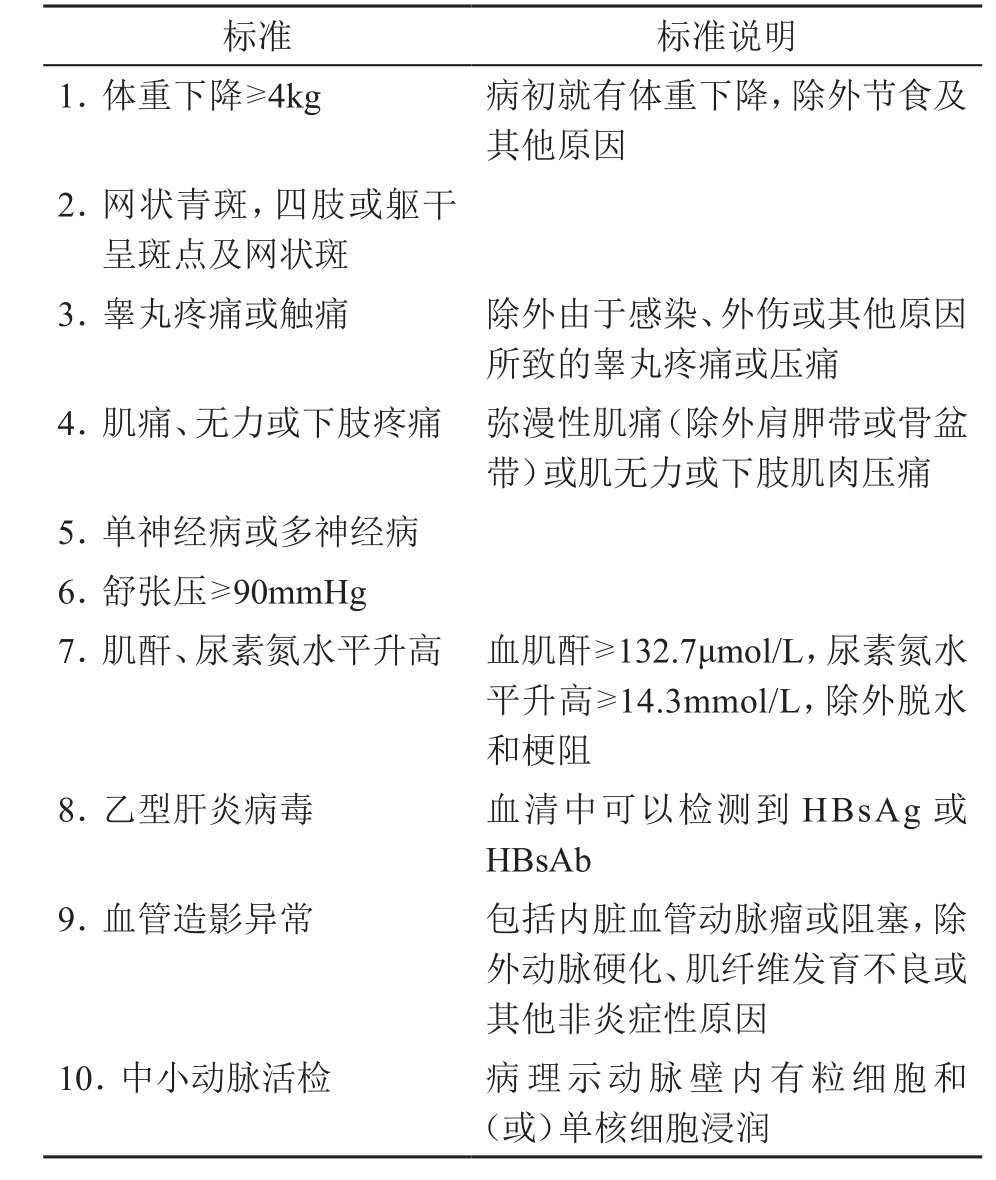
\includegraphics[width=3.3125in,height=3.91667in]{./images/Image00502.jpg}
\end{table}

使用激素时应随时注意激素的副作用如感染、低血钾、水钠潴留、高血压、糖尿病、骨质疏松等。但无论如何,糖皮质激素的治疗是PNA治疗的根基。尽管目前的研究尚无比较单用激素以及联合另一种药物通常是细胞毒类药物的治疗差异,但临床上如果重要脏器受到威胁,控制病情所需要的激素剂量过大,通常有经验的医生会在激素的基础上加用另一种药物。

\paragraph{免疫抑制剂}

①环磷酰胺:通常是在治疗PAN时细胞毒类药物的首选,环磷酰胺每日2~3mg/kg(多数患者符合这个标准),予以口服或静脉用药,把剂量调整至维持白细胞在(3.0~3.5)×
10\textsuperscript{9}
/L,完全缓解后要继续治疗并逐渐减量,大多数风湿科医生一旦使用该药,通常会间断性连续使用1~2年。该使用方法目前认为毒性相对较小,且疗效可能与持续小剂量口服相当。治疗过程中要注意药物的副作用,如:骨髓抑制、出血性膀胱炎等。②其他免疫抑制剂:甲氨蝶呤、硫唑嘌呤、苯丁酸氮芥、环孢素,秋水仙碱等。

\paragraph{抗病毒治疗}

近年来的观察发现,抗病毒药物拉米夫定(lamivudine,100mg/d)治疗对于HBV相关的PNA已有明确效果,同时包括最初的激素(泼尼松)治疗(1mg/kg•d)。在乙型和丙型肝炎相关的血管炎患者使用干扰素治疗,也呈现令人鼓舞的结果。

\paragraph{其他治疗以及对症治疗}

尽管使用激素及免疫抑制剂使PNA的预后明显改善,但仍然有部分患者严重的器官损害得不到控制,近年来一些新的治疗手段已经应用于临床,并取得一定的疗效,包括:静脉注射免疫球蛋白、单克隆抗体、血浆置换。

对症治疗措施:包括抗高血压、维持水电解质平衡、注意肾脏损害、控制心衰(洋地黄化)和输血。PNA血管内膜的炎症以及糖皮质激素的使用可以增加潜在的血管收缩能力及血小板的聚集,故应使用抗凝药物和血管扩张药物如:阿司匹林、尼莫地平等。出现肠道溃疡及穿孔时需要求助外科治疗。

\subsection{预后}

PAN的预后及治疗策略的评估:在应用激素和免疫抑制剂治疗之前,PAN几乎是致死性的疾病,5年生存率约10\%,激素治疗使其5年生存率上升至50\%左右,激素和免疫抑制剂(环磷酰胺)使5年生存率超过80\%。就临床表现有5个与高死亡率相关的因素FFS(five
factor score)方法评估PAN:①蛋白尿>
1g/24h;②肾功能不全;③心脏损害;④消化系统受累;⑤中枢神经系统受累。以上5项满足1项计1分。FFS
= 0,其5年死亡率为12\%;FFS = 1,其5年死亡率为26\%;FFS =
2,其5年死亡率为46\%。该评估方法的精神是:重要脏器受累的数目及程度决定了系统性血管炎的预后。这符合临床思维的常识,其对该病的预后、治疗方案的选择有一定的示范作用和参考价值。

\protect\hypertarget{text00349.html}{}{}

\hypertarget{text00349.htmlux5cux23CHP14-2-5}{}
参 考 文 献

1. Fraenkel-Rubin M,Ergas D,Sthoeger ZM. Limited polyarteritis nodosa
of the male and female reproductive systems:diagnostic and therapeutic
approach. Ann Rheum Dis,2002,61(4):362-364

2. Giouleme O,Mpoumponaris A,Aslanidis S,et al. Polyarteritis nodosa
in a patient with type 1 autoimmune hepatitis. South Med
J,2011,104(1):49-52

3. Guillevin L,Mahr A,Callard P,et al. Hepatitis B virusassociated
polyarteritis nodosa:clinical characteristics,outcome,and impact of
treatment in 115 patients. Medicine
(Baltimore),2005,84(5):313-322

4. Bourgarit A,Le Toumelin P,Pagnoux C,et al. Deaths occurring during
the first year after treatment onset for polyarteritis
nodosa,microscopic polyangiitis,and Churg-Strauss syndrome:a
retrospective analysis of causes and factors predictive of mortality
based on 595 patients. Medicine(Baltimore),2005,84(5):323-330

5. Buonuomo PS,El Hachem M,Callea F. Necrosis of the tongue as first
symptom of (PAN):unusual presentation of a rare disease in children.
Rheumatol Int,2010,7:456

\protect\hypertarget{text00350.html}{}{}

\chapter{特发性炎症性肌病}

特发性炎症性肌病(idiopathic inflammatory
myositis,IIM)是一组病因未明的以四肢近端肌无力为主的骨骼肌非化脓性炎症性疾病,其共同表现为对称性近端肌无力。目前将其分为七类:①多发性肌炎(polymyositis,PM);②皮肌炎(dermatomyositis,DM);③儿童皮肌炎;④恶性肿瘤相关性PM或DM;⑤其他结缔组织病伴发PM或DM;⑥包涵体肌炎(inclusion
body myositis,IBM);⑦无肌病性皮肌炎(amyopathic
dermatomyositis)。我国PM/DM临床上并不少见,但发病率尚不清。男女发病率比为1∶2,可发生在任何年龄,呈双峰型,第一高峰在儿童期,10~15岁,第二高峰在45~60岁。PM/DM临床表现多样,本章重点讨论PM和DM的急症表现及处理。

\subsection{病因与发病机制}

\subsubsection{病因}

病因尚不清楚,其发生可能与遗传、感染、药物、免疫和应激等多种因素有关。

\paragraph{遗传}

家系研究和候选基因方法提示该类疾病有遗传因素的参与。已证明HLA基因、TCR基因、细胞因子及细胞因子受体基因、Fc受体基因等与该类疾病相关,有研究发现HLA-B8增加PM/DM患病风险。

\paragraph{免疫}

本病常伴其他自身免疫性疾病如桥本甲状腺炎、Graves病、1型糖尿病、重症肌无力等。体液免疫异常如血清中可以检测出抗Jo-1抗体、抗Ro/La抗体;血清中IL-1α、IL-2受体的存在;皮肤、肌肉的血管内膜有免疫球蛋白、补体沉积等。不少病例伴有多克隆高球蛋白病。细胞免疫方面的证据,包括可检测到外周单核细胞对T淋巴细胞、肌肉组织增殖反应的改变;肌细胞周围以活化的CD8\textsuperscript{+}
T细胞为主的大量单核细胞的浸润等。

\paragraph{感染}

有证据提示炎性肌病的发生和感染,如寄生虫、病毒、细菌、真菌等有关。弓形体和螺旋体感染后,患者可以出现PM/DM的临床表现;一些反转录病毒如HIV、HTLV-1与肌炎的发生具有相关性;腺病毒在包涵体肌炎、柯萨奇病毒在慢性肌病均曾检出,但在典型的PM、DM患者中则罕见。虽然如此,感染在炎性肌病的作用,尚待进一步研究证实。

\paragraph{药物、肿瘤等其他因素}

临床中发现某些药物可以引起肌炎的症状,如氯喹、秋水仙碱、乙醇、西咪替丁、青霉胺、可卡因及某些降脂药等,长期应用糖皮质激素可以引起“类固醇肌病”。研究提示,DM合并恶性肿瘤的危险性比正常人群增加3~6倍,而PM则增加1.4~2倍。其他因素如过度劳累、情绪激动等可能也会诱发肌炎的发生。

\subsubsection{发病机制}

目前普遍认为本病是免疫损伤导致的自身免疫性疾病。细胞免疫异常和体液免疫异常在不同类型炎性肌病中表现不同。细胞免疫在PM的发病机制中占主要的地位,肌纤维细胞在某些刺激下(如病毒、细菌感染)表达MHC-Ⅰ类抗原,当与抗原结合后,可以促使T淋巴细胞活化增殖,发生免疫反应导致局部损伤。DM的发病机制更倾向于体液免疫,其肌肉损伤常继发于小血管病变,该病变可能与膜攻击复合物在血管壁的沉着造成血管内皮细胞损伤有关。同时,PM/DM外周血中和肌组织中发现高水平的免疫球蛋白,造成机体的损伤。

\subsection{诊断}

\subsubsection{临床表现特点}

\paragraph{全身表现}

可有发热,晨僵,疲乏,厌食,消瘦、全身不适等非特异性症状。

\paragraph{肌肉}

本病累及横纹肌,以对称性肢体近端肌无力为其临床特点,常常发病隐匿,个别患者急性起病。早期可有肌肉肿胀、压痛,随病情进展,几乎所有患者均出现不同程度的肌无力,晚期以肌萎缩、纤维化为主。肩带肌和骨盆肌受累的表现较为突出,如上肢不能上举,不能梳头、穿衣;抬腿不能或困难,坐下或下蹲后起立困难等。约一半患者出现颈部肌无力,躯干肌肉受累致平卧起床困难,眼肌、面部及球肌受累罕见。颈深肌群的受累使食管不协调运动,出现吞咽困难、进食呛咳,重症者导致反复吸入性肺炎、肺脓肿,甚至发生急性呼吸窘迫综合征(ARDS)。胸腔肌和膈肌受累出现呼吸表浅、呼吸困难,并引起急性呼吸功能不全。亦可出现急性横纹肌溶解症。

\paragraph{皮肌炎皮肤损害}

典型的DM皮肤表现为:①Gottron皮疹:出现在关节伸面皮肤的紫红色斑丘疹,表面扁平且边缘不整,尤其在掌指关节和指间关节多见,为DM的特征性皮疹。②眶周红斑:表现为眶周水肿性紫红色斑,外周色淡,像“熊猫眼”,仅上眼睑受累的,称“向阳性皮疹”,也是DM的特征性皮疹。③“V领”征及“披肩”征:指颈部、胸前V形区、后背上部呈现毛细血管扩张样红斑,可伴有有皮肤萎缩、色素脱失或沉着等。DM非典型的皮肤损害包括甲周红斑、“技工手”、皮肤钙化及局部溃疡等。

\paragraph{关节}

关节痛可见于1/4的患者,多发生于疾病的早期,常对称性累及手、腕、足和踝关节,非侵蚀性,明显滑膜炎少见,晨僵多见,对糖皮质激素治疗反应好。

\paragraph{肺部}

约30\%患者有间质性肺疾病,少数患者出现肺动脉高压。累及食管出现吞咽困难者,可引起吸入性肺炎。

\paragraph{消化系统}

15\%~50\%的患者有食管功能异常,最常见症状为吞咽困难,为舌、咽、食管横纹肌无力所致,造成反流性食管炎。严重胃麻痹罕见,胃肠道炎症还可引起腹痛、便秘和腹泻。胃肠道血管炎可致肠出血甚至肠穿孔,表现为腹痛、血便等症状。

\paragraph{心脏}

70\%患者在病程中可累及心脏,多数无临床症状,不需处理。常见心脏表现有心律失常、传导阻滞、心包炎、心肌炎、心肌梗死、心力衰竭,也可表现为心脏瓣膜病、冠状动脉炎等。与肺部病变同时出现者预后更差。

\paragraph{恶性肿瘤相关性肌炎}

恶性肿瘤与肌炎的关系尚不明确,多认为肌炎患者恶性肿瘤的发生率增加,DM多于PM,特别是在肌炎诊断后的5年之内。种类与同年龄段人群所罹患肿瘤相似。年老发病、男性可为独立危险因素,间质性肺病可能为肿瘤发生的保护性因素。

\paragraph{无肌病性皮肌炎}

指有些患者皮肤病变具有典型皮肌炎的特点,而没有明显的肌肉受累症状,疲乏可成为突出表现。检查可提示轻微的、亚临床肌病性异常改变。很多患者如不治疗,数月后可出现明显的肌肉病变。该类型皮肌炎常合并肺部病变,预后较差。

\paragraph{抗合成酶综合征}

多发生于中年女性,除炎症性肌病外,还表现为低热、间质性肺病,雷诺现象,技工手和手小关节炎。该综合征的特点为患者的血清中出现抗合成酶抗体。有些患者以雷诺现象或肺部病变为突出表现,可先于或掩盖肌病。

\paragraph{幼年型 PM/DM}

儿童DM多于PM,起病急,肌肉水肿、疼痛明显,可有视网膜血管炎,并常伴有胃肠出血、黏膜坏死,出现呕血或黑便,甚至穿孔。疾病后期,皮下、肌肉钙质沉着,肌肉萎缩。

\paragraph{包涵体肌炎}

类似慢性多肌炎,多发生于老年男性,患者远端肌无力突出,特别是前臂和手无力明显。发病潜隐,从起病到诊断需数月至数年,多数患者没有肌肉外表现,可出现吞咽困难。

\subsubsection{辅助检查}

\paragraph{一般检查}

大部分患者出现红细胞沉降率增快、C反应蛋白升高,有些会出现白细胞轻度增高和贫血。部分肌炎患者可有血肌红蛋白、尿肌红蛋白升高,急性广泛的肌肉破坏甚至可以出现肌红蛋白尿。肌肉病变时可以有血肌酸升高,而肌酐不升高,这在PM/DM中不特异。

\paragraph{肌酶谱检查}

血清肌酶谱检查是本病最常用的实验室检查方法,其中肌酸磷酸激酶(CK)的改变对肌炎诊断及其活动性判断最为敏感和特异,是肌肉炎症损伤的标志酶。但多种组织(如心肌、肝、脑等)损伤时都会有CK释放入血,可用CK同工酶来区别,如CK-MM多在肌炎时升高,CK-MB心肌受累时升高明显。需要注意的是疾病晚期出现肌萎缩的患者,CK可以无明显升高,包涵体肌炎患者CK也可正常或轻度偏高。碳酸酐酶Ⅲ是唯一存在于骨骼肌中的同工酶,它对PM及其他骨骼肌病变疾病的诊断较有特异性。血清醛缩酶(ALD)升高也可以协助诊断,但特异性不及CK。天冬氨酸转氨酶(AST)、丙氨酸转氨酶(ALT)及乳酸脱氢酶(LDH)等因在多种组织中存在,只有在排除肝脏、心肌等损伤后方可提示骨骼肌病变,只作为诊断参考依据。

\paragraph{自身抗体}

肌炎患者可以出现多种自身抗体。抗核抗体阳性率为38.5\%~80\%,以斑点型最多见。肌炎诊断中特异的自身抗体包括:①抗合成酶抗体,包括抗JO-1、抗PL-7、抗PL-12、抗OJ和抗EJ等抗体,以抗JO-1抗体阳性率最高,临床应用最多,特别是在有肺间质病变者。②抗SRP抗体见于少部分起病急、肌炎重、心脏受累且治疗反应差的患者。③抗MI-2主要出现在有V字征、披肩征的DM患者中。部分患者血中可检测出抗肌红蛋白抗体、抗肌钙蛋白抗体、抗肌球蛋白抗体、抗骨骼肌抗体等非特异性抗体。此外,一些肌炎相关的抗体如抗Scl-70抗体出现在合并系统性硬化症者,抗SSA、抗SSB抗体出现在伴干燥综合征者,抗RNP抗体则在混合性结缔组织病常见。

\paragraph{肌电图(EMG)}

肌电图检查可作为肌炎诊断和确定活动性的重要指标,多数为肌源性改变,少数也可以为神经源性损伤或两者兼有。EMG异常改变包括:自发性肌纤颤形成,出现锯齿形电位;运动电位时相缩短,多相波电位增加;平均电压波幅下降。恢复期纤颤电位消失和运动单位平均时限恢复正常可以作为判断治疗的客观指标。包涵体肌炎约50\%为神经源性改变或肌源性和神经源性两者兼有。

\paragraph{组织活检}

肌肉活检和皮肤活检是确诊炎性肌病重要手段。肌活检做多部位活检可提高阳性率,常选择肌电图出现异常部位的对侧或MRI提示异常的部位取材,但仍有10\%~25\%患者表现为非特异性炎症改变。病理改变包括:肌细胞肿胀、空泡样变,并有不同程度的再生;肌纤维变性、坏死,肌横纹消失;肌束间纤维化,成纤维细胞增生,伴有炎症细胞浸润或钙化灶形成;肌间隙小血管周围炎症细胞浸润,血管内膜增厚等等。皮肌炎皮肤病理表现有基底细胞空泡变性,基底膜、棘层增厚,并有黏多糖沉积及炎性细胞浸润等等非特异的改变。包涵体肌炎肌活检时尚有特征性改变,即在受累肌细胞胞浆或胞核内出现嗜酸性的包涵体。注意少数有肌炎典型表现而肌活检无明显异常者易合并肿瘤。

\paragraph{影像学检查}

影像学技术是用于协助肌炎诊断的无创性手段。磁共振成像(MRI)应用最多,在肌肉炎症部位显示高密度T\textsubscript{2}
波,可以发现肌肉软组织早期、微细的病变,有时甚至比EMG更能精确的确定活检部位,并可半定量分析病变程度、对治疗进行随访观察。超声检查可以发现炎症、水肿、萎缩部位肌束的异常回声。此外,各种影像学检查对于及时发现恶性肿瘤、进行相关辅助检查也发挥一定作用。

\subsubsection{诊断标准}

目前尚无一致公认的诊断标准,临床应用较多的有1975年Bohn、Peter诊断标准、1982年Maddin诊断标准和WHO诊断标准等。其中1975年由Bohn和Peter提出的PM及DM的诊断标准,到目前仍被广泛应用:①对称性、进行性的近端肌无力,伴或不伴呼吸道、食管肌肉的损害;②肌活检异常:肌细胞或肌纤维有不同程度变性、坏死、再生等改变,伴或不伴筋膜周围的肌萎缩和炎症反应;③血清肌酶升高:如肌酸磷酸激酶及其同工酶、醛缩酶、ALT、AST、乳酸脱氢酶;④肌电图提示肌源性损害:表现为时限短、波幅低多相运动电位,纤颤波,插入性激惹和异常的高频放电;⑤皮肤损害:眼睑呈淡紫色、眶周水肿;掌指关节及近端指间关节背面鳞屑性红色皮疹(Gottron征);颈前、上胸部、颈后背上部出现的红斑性皮疹。

凡具有①②③④者可确诊为PM,具备①~④项中的三项可能为PM,只具备二项为疑诊PM。具备第⑤条,再加上三项或者四项可确诊为DM。第⑤条,加上二项可能为DM。第⑤条,加上一项为可疑DM。

\subsection{治疗}

\subsubsection{一般治疗}

该病为慢性疾病过程,要给予综合治疗包括药物、心理、物理治疗等。急性期注意休息,加强护理,肢体做适当被动运动,以防肌肉挛缩,并给予高蛋白、高热量饮食,伴有严重吞咽困难者,应以流质饮食为主,必要时可鼻饲,防止出现吸入性肺炎。恢复期需加强肌肉锻炼,可配合物理治疗以防治肌肉萎缩。皮肌炎患者还应注意避免日晒。

\subsubsection{药物治疗}

\paragraph{糖皮质激素}

是治疗多发性肌炎和皮肌炎的首选药。泼尼松成人起始剂量为1~2mg/(kg•d),儿童1.5~2.5mg/(kg•d),否则易复发。病情控制后5~10mg维持治疗数月或数年,总疗程不少于2年。出现严重脏器受累者或进行性加重的肌无力,需采用甲泼尼龙每天1g静脉注射,连续3天,之后以口服泼尼松60mg/天维持。治疗中应注意出现“类固醇肌病”,其表现与多肌炎类似,易与肌炎加重混淆,鉴别方法为观测治疗中CK是否增加、激素减量症状是否好转以及肌电图改变。

\paragraph{免疫抑制剂}

足量泼尼松治疗4~6个月病情无改善或加重者,及糖皮质激素副作用明显或不能耐受者,应联合应用免疫抑制剂。常用的有硫唑嘌呤、甲氨蝶呤、环磷酰胺和环孢霉素。硫唑嘌呤:临床应用较多,每日1~2mg/kg,不良反应发生率较低,主要有骨髓抑制、肝酶升高等。甲氨蝶呤:每周7.5~15mg,口服或静脉注射同效。其疗效与硫唑嘌呤类似且起效相对较快,但需注意由于存在致肺纤维化的副作用,应尽量避免应用于已经出现间质性肺病或抗Jo-1抗体阳性者。环磷酰胺:每日1~2mg/kg口服,或0.85g/1.7m\textsuperscript{2}
体表面积,每月一次静脉注射,活动期可静脉冲击治疗,对间质性肺病患者有效。副作用包括性腺抑制、骨髓抑制及肝损害,出血性膀胱炎、恶性病变少见。环孢素A:每日2~3.5mg/kg,副作用有多毛、升高血压、高血钾、肾损害等,随剂量减少而降低,疗效也随之下降。

\paragraph{抗疟药}

用于控制皮肌炎的皮肤病变及减少皮质激素用量。氯喹推荐剂量250mg/d,羟氯喹200~400mg/d,4~6个月后减量维持,每周2次给药。注意用药期间行眼科检查。

\paragraph{静脉免疫球蛋白(IVIg)}

人血免疫球蛋白IgG
1000mg/(kg•d),连续3天静脉注射。为避免升高血压、栓塞等副作用,近年多主张300~400mg/(kg•d),连续3~5天静脉注射,以后每月一次维持治疗,预防复发。

\subsubsection{其他}

包括血浆置换、全身性放射治疗等,对某些患者有一定疗效。近几年,霉酚酸酯和生物学制剂如抗肿瘤坏死因子单克隆抗体等也开始试用于本病的治疗,临床疗效有待进一步证实。

\subsubsection{PM和DM各个系统危重急症处理}

\hypertarget{text00350.htmlux5cux23CHP14-3-3-4-1}{}
(一) 呼吸系统急症

\paragraph{急性间质性肺炎}

患者可于疾病的任何一个时期出现间质性肺病(ILD),临床表现和预后差异大。急性起病者表现为发热、咳嗽、呼吸困难、发绀,查体可闻及肺底Velcro啰音,影像学表现为弥漫性肺泡间质浸润,间质纤维化时呈条索状、网格状改变,晚期可见蜂窝状阴影、肺动脉段增宽等。慢性起病者,临床表现隐匿,缓慢出现进行性加重的气短、发绀等症状。表现抗合成酶综合征时尚有雷诺现象、关节痛、技工手等,不能有效控制者最终多死于呼吸衰竭。

炎性肌病患者ILD可分为三种类型:①急性间质性肺炎(Hamman-Rich样)型:呼吸困难快速进展,ILD症状出现3个月内出现呼吸衰竭,需要机械通气支持治疗。②缓慢进展型:肺部ILD症状进行性发展,但速度不及急性间质性肺炎型。③无症状型:没有肺部症状和体征,胸片或肺功能检查提示肺部病变存在。

肺功能检查往往有通气和(或)弥散功能障碍,常先于X线片出现异常,可以列为常规检查。支气管镜和开胸肺活检对明确组织病理类型、指导治疗、判断预后有较好作用,但为创伤性检查不易被患者接受。根据活检病理不同,肺部病变可分为四种类型:闭塞性机化性细支气管炎;普通型间质性肺炎;弥漫性肺泡损伤和非特异性间质性肺炎。除闭塞性机化性细支气管炎治疗效果较好以外,其他类型的间质性肺疾病均对治疗反应不好,预后较差。

处理:急性间质性肺炎及肺部纤维化迅速进展常常是本病死亡的重要原因之一,一旦发现,需及时处理。初始治疗包括大剂量糖皮质激素口服(相当于泼尼松60~80mg/d),不合并感染、出现呼吸困难的患者可用甲强龙冲击治疗。早期即应开始应用免疫抑制剂,可选用环磷酰胺、硫唑嘌呤、环孢素等,剂量如上述。也可应用IVIg。

\paragraph{吸入性肺炎}

可见于颈深肌群受累者,由于食管蠕动障碍,引起吞咽困难、进食呛咳、胃食管反流,继而引起吸入性肺炎、肺脓肿,甚至可能发生呼吸衰竭或急性呼吸窘迫综合征(ARDS)。

当胃内容物误吸入气管后,胃酸可立即引起气道和肺泡化学性灼伤,产生急性肺部炎症反应。胃酸刺激支气管引起管壁强烈痉挛,随后产生支气管上皮的急性炎症反应和支气管周围炎性浸润。进入肺泡的胃液迅速扩散至肺组织,引起肺泡上皮细胞破坏、变性,并累及毛细血管壁,使血管壁通透性增加,血管内液体渗出,引起水肿及出血性肺炎。同时由于肺泡毛细血管膜的破坏,形成间质性肺水肿。数日后肺泡内水肿和出血逐渐吸收,并被透明膜所代替。久之可形成肺纤维化。吸入的食物若将咽部定植菌带入肺内,可导致继发性细菌感染,形成肺脓肿。同时,肺水肿使肺组织弹性减弱,顺应性降低,肺容量减少,加之肺泡表面活性物质减少,使小气道闭合,肺泡萎陷引起微肺不张,均可产生通气不足、通气/血流比例失调和静动脉血分流增加,导致低氧血症或伴代谢性酸中毒。血管内液大量渗出或反向性血管扩张,亦可产生低血压。

其严重程度与胃液中盐酸浓度、吸入量以及在肺内的分布情况有关。吸入胃酸的pH≤2.5时,吸入量25ml即能引起严重的肺组织损伤。动物实验中证实,吸入pH
< 1.5的液体3ml/kg体重时可致死。吸入液的分布范围越广泛,损害越严重。

处理:紧急情况下,应立即给予高浓度氧吸入,应用纤维支气管镜或气管插管将异物吸出,出现急性呼吸窘迫综合征时,加用呼气末正压通气辅助治疗。应用白蛋白或低分子右旋糖酐等纠正血容量不足。为避免左心室负担过重和胶体液渗入肺间质,可使用利尿剂。对于糖皮质激素,有学者认为在吸入12小时内大剂量使用,有利于肺部炎症的吸收,但亦有持反对意见者。抗生素只用于控制继发性感染,不主张用于预防细菌性感染。

\paragraph{呼吸肌无力}

胸腔肌和膈肌受累时,出现呼吸表浅、呼吸困难,重症者可引起急性呼吸衰竭(Ⅱ型)。

处理:大剂量糖皮质激素为首选,一般成人剂量1~2mg/(kg•d),儿童1.5~2.5mg/(kg•d),也可试用大剂量甲泼尼龙冲击治疗,及早给予免疫抑制剂应用。同时低浓度氧疗及纠正急性呼吸衰竭引起的酸碱失衡等。对于病情危重,症状持续不缓解,机体出现严重的通气功能障碍时,可暂时呼吸机辅助呼吸,等待呼吸肌功能的恢复。

\paragraph{肺动脉高压}

较为罕见,表现为进行性加重的呼吸困难,并可出现肺心病的临床表现。病理基础为肺小动脉壁增厚和管腔狭窄。胸部X线检查示肺动脉段扩张,不伴肺纤维化时肺野清晰。多普勒超声为发现肺动脉高压的一简便有效的检查方法。伴肺动脉高压的肌炎患者预后差。

处理:类似于特发性肺动脉高压,如利尿、华法林抗凝。硝苯地平及其他钙离子拮抗剂可改善血流动力学异常,连续静脉注射前列环素可能增加生存时间。有报道糖皮质激素联合免疫抑制剂如环磷酰胺可改善预后。

\hypertarget{text00350.htmlux5cux23CHP14-3-3-4-2}{}
(二) 消化系统急症

\paragraph{严重食管功能障碍}

食管上段横纹肌受累引起吞咽困难,饮水发生呛咳、液体经鼻孔流出;食管下段受累引起反酸、食管炎、咽下困难。严重食管受累者,完全不能经口进食或经胃管肠道营养,引起严重营养不良,吸入性肺炎、肺脓肿及呼吸衰竭等。食管受累被认为是PM和DM患者死亡的一个重要因素,常常提示预后不良。

处理:首选大剂量激素应用,因不能经口进食,可静脉应用甲泼尼龙。也可应用IVIg,尤其适用于激素抵抗患者。可以尽早行经皮内镜胃造瘘术进行肠道喂养。免疫抑制剂尽早使用,可选环磷酰胺、硫唑嘌呤、环孢素等,剂量如上述。

\paragraph{胃肠道血管炎及穿孔}

胃肠道血管炎多发生在儿童DM中,成人DM亦可见,表现为腹痛、血便等。并发穿孔则腹痛加重,出现腹膜炎表现,CT等影像学检查可发现腹腔内游离气体、坏死,腹膜后脓肿等。穿孔部位可发生于食管、胃、十二指肠、结肠及盲肠,病理活检可见动脉、静脉内膜增厚,纤维蛋白血栓所致的血管闭塞,淋巴细胞浸润破坏各种管径的静脉等表现。

处理:重点在于诊断,当幼年DM患者出现腹部不适、疼痛、血便时,需警惕胃肠道血管炎或并发溃疡、穿孔的可能。当血管炎未合并溃疡、穿孔时,糖皮质激素为首选,儿童1.5~2.5mg/(kg•d)。一旦穿孔,则需立即外科手术,清创坏死组织,修补穿孔。

\hypertarget{text00350.htmlux5cux23CHP14-3-3-4-3}{}
(三) 心血管系统急症

\paragraph{心肌炎}

尸体解剖发现30\%炎性肌病患者存在心肌炎,心肌内有炎症细胞浸润,间质水肿和变性,局灶性坏死,心室肥厚,可出现心律失常、充血性心力衰竭,亦可出现心包炎。可出现心电图异常、心肌酶学升高以及多普勒超声检查异常。肌钙蛋白具较高的心肌特异性,可能作为评价心肌炎的一有益指标,近年来出现的心血管磁共振成像为一有价值的检查手段。

\paragraph{充血性心力衰竭}

多发生于炎性肌病活动性病变患者,也偶见于横纹肌炎症不明显者、免疫抑制剂治疗期间甚至缓解期的患者。临床表现同于其他疾病引起的充血性心力衰竭。

处理:急性期注意卧床休息,加强营养。针对心衰应用血管扩张剂、利尿剂,慎用洋地黄类药物,并积极处理各种心律失常。出现严重的房室传导阻滞应安装临时起搏器。轻症患者可口服泼尼松40~60mg/d,严重者给予甲泼尼龙1g/d,共3天,早期联用免疫抑制剂,如环磷酰胺、甲氨蝶呤、硫唑嘌呤等有助于改善预后。

\hypertarget{text00350.htmlux5cux23CHP14-3-3-4-4}{}
(四) 急性横纹肌溶解综合征

横纹肌溶解综合征临床表现为肌肉剧痛
,压痛和肌肿胀。血清CK水平可显著升高,大量肌肉坏死可引起低钙血症,高尿酸血症,高钾血症和肌红蛋白尿。急性肾小管坏死所致肾衰竭为横纹肌溶解症最严重的并发症,也可发生急性尿酸性肾病。

处理:主要是支持治疗。肌红蛋白尿时可应用利尿剂,以预防肾衰竭,存在尿酸性肾病时要碱化尿液,扩容,注意电解质紊乱的防治。出现急性肾衰竭时给予基础治疗如保持水、电解质平衡、营养支持、控制高血压、血液净化等。

\hypertarget{text00350.htmlux5cux23CHP14-3-3-4-5}{}
(五) 肾脏急症

肾脏病变很少见
,极少数暴发性起病者,多由于横纹肌溶解,表现为急性肾小管坏死或急性尿酸性肾病,可导致急性肾衰竭。

处理:同上述对横纹肌溶解综合征的治疗。

\protect\hypertarget{text00351.html}{}{}

\hypertarget{text00351.htmlux5cux23CHP14-3-4}{}
参 考 文 献

1. Wang IJ,Hsu WM,Shun CT,et al. Juvenile dermatomyositis complicated
with vasculitis and duodenal perforation. J formos Med
Assoc,2001,100(12):844-846

2. Yusuf Yazici MD,Lawrence J,Kagen MD. Clinical presentation of the
idiopathic inflammatory myopathies. Rheum Dis Clin N
Am,2002,28:823-832

3. Harris. Kelley's Textbook of Rheumatology. 8th ed. 2008

\protect\hypertarget{text00352.html}{}{}

\chapter{系统性硬皮病}

硬皮病(scleroderma)是一种以皮肤炎性、变性、增厚和纤维化进而硬化和萎缩为特征的结缔组织病。其中系统性硬皮病(systemic
sclerosis,SSc)除皮肤、滑膜、指(趾)动脉出现退行性病变外,消化道、肺、心脏和肾等内脏器官也可受累。此病在世界范围内呈散发性,与季节、地理和社会经济状况无关。发病年龄多在30~55岁之间,女性高于男性,男女之比为1∶7~12,以常见于生育中、后期年龄组的女性,20岁以下患SSc者很少见。近年来此病发病率有上升的趋势,约为0.019\%~0.025\%。

\subsection{病因与发病机制}

\subsubsection{病因}

SSc的病因仍不明确,可能在遗传、环境因素(病毒感染、化学物质如硅等)、女性激素、细胞及体液免疫异常等因素作用下,成纤维细胞合成并分泌胶原增加,导致皮肤和内脏的纤维化。

化学物质或病毒感染是影响疾病易感性的环境因素。常暴露于二氧化硅的人群患此病相对危险性增高。有报道表明,暴露于有机溶剂、生物源性氨基酸和尿素甲醛可引起系统性硬化。也有报道吸烟、饮酒和饲养宠物可增加患SSc的危险性。病毒与SSc自身抗原的同源性提示病毒对疾病的易感性有潜在的作用。猫科肉瘤病毒和巨细胞病毒的DNA拓扑异构酶与P30GAG蛋白有同源性。对SSc较特异的PM-Scl抗原区与SV-40大T抗原及人免疫缺陷病毒tat蛋白有同源性。Ⅱ型单纯病毒的CP4蛋白与U1RNP(可能为SSc的早期抗原)共有一段氨基酸片段;Ⅰ型单纯疱疹病毒编码的病毒外壳蛋白及EB病毒的核抗原1与原纤维蛋白有同源性。

遗传对SSc的发病没有很强的关联。SSc与HLA-DQA2、CAA无效等位基因,T细胞抗原受体基因的等位基因C72有较弱的相关性,在SSc中,P-450酶活性降低。与RA及SLE不同,同一家族中患SSc的人很少超过一个,也很少有患病的一级血缘关系。单卵及双卵双生同胞的发病率相同。

\subsubsection{发病机制}

SSc的发病机制尚不清楚,可能是由于免疫系统功能失调,激活、分泌多种自身抗体、细胞因子等引起血管内皮细胞损伤和活化,进而刺激成纤维细胞合成胶原的功能异常,导致血管壁和组织的纤维化。小血管内皮细胞之间、成纤维细胞和免疫系统的相互作用造成了SSc的发病。

\subsubsection{病理}

广泛的小血管病变和纤维化的发生是SSc区别于其他结缔组织病的主要特点,皮肤和内脏都可出现并引起器官功能障碍的临床症状。血管病变和纤维化是由自身免疫反应所引起。就指(趾)雷诺现象的病理改变而言,表现为指(趾)动脉显著的内膜胶原和基质增殖,中膜改变不明显,约40\%有外膜纤维化,75\%以上造成动脉管腔严重狭窄。小血管病变首先是小动脉、微动脉和毛细血管增生和闭塞过程。这种病变始于内皮层的活化和损伤。细胞支架结构内纤维丝非特异性崩溃,继而造成细胞质空泡形成及细胞膜的水肿,失去细胞间紧密的连接,内皮层脱落到血管腔内,最终结果是内皮层细胞的消失。小血管内膜基质层疏松纤维中平滑肌样肌内膜细胞增生,血管腔狭窄不断进展。而内皮细胞损伤引起血小板活化和血栓形成后又加重了这种狭窄。血小板活化后能释放介质,如血小板衍生生长因子(PDGF)、血栓素A2,继而诱导血管收缩并刺激内皮细胞和成纤维细胞的生长,使基质膜增厚和修复,真皮内血管周围水肿、蛋白质物质渗出、血管内和血管周围纤维蛋白沉积,所有这些改变都会减少营养物质通过血管的运送。

SSc中的纤维化是由于成纤维细胞活化导致胶原、纤维连接素和氨基葡萄糖的沉积增加所造成的。皮肤的皮下结缔组织和真皮下纤维化都非常明显。Ⅰ、Ⅲ、Ⅴ和Ⅵ型胶原的mRNA及蛋白的合成均增加。其他支持成纤维细胞活化的证据是成纤维细胞表面的HLA-DR分子和ICAM-1表达增加。在SSc患者中,临床表现正常的皮肤也可见到成纤维细胞的活化,但前胶原酶ImRNA的表达增加并不出现纤维化。纤维化可能表明SSc患者成纤维细胞活化的最终结果。

\subsection{诊断}

\subsubsection{临床表现特点}

SSc起病隐匿,雷诺现象常为本病的首发症状,90\%以上先于皮肤病变数月至数年(大部分5年内)。

\paragraph{雷诺现象}

是指患者在受凉或紧张的刺激后,肢端细动脉痉挛,使手指(足趾)皮肤突然出现苍白,相继出现皮肤变紫、变红,伴局部发冷感觉异常和疼痛等短暂的临床现象。普通人群中4\%~15\%的人有雷诺现象,但大多数均较轻,而且没有血管结构损伤和组织局部缺血。SSc患者中90\%以上有雷诺现象,随之可造成手指组织纤维化、指(趾)硬化及溃疡、偶发的局部缺血,这些与指(趾)缩短均有关。雷诺现象除血管痉挛外,还有血管内壁纤维化引起的血管闭塞、血小板活化和纤维蛋白沉积。硬皮病也可以有系统性雷诺现象的发生,它是一种泛发性的血管痉挛,包括侵犯肾、肺、心脏血管循环末端动脉的血管病。

\paragraph{皮肤病变}

为本病标记性特点,呈对称性。一般先见于手指及面部,然后向躯干蔓延。典型皮肤病变一般经过3个时期:①肿胀期:在疾病的早期,皮肤显示轻度红肿,部分患者有红斑、瘙痒。患者感觉进行性皮肤增厚和屈曲度减弱。手和手指、前臂出现双侧对称性无痛性水肿,手指肿胀发紫,状如腊肠。水肿持续几周或几个月后渐渐进入硬化期。②硬化期:皮肤逐渐变厚、发硬,手指像被皮革裹住,双手不能握紧拳头。皮肤病变可以逐渐向手臂、颈部、上胸部、腹部及背部蔓延,两条腿很少受累。面部皮肤受损造成正常面纹消失,使面容刻板,鼻尖变小,鼻翼萎缩变软,嘴唇变薄、内收,口周有皱褶,张口度变小,称“面具脸”,为本病特征性表现之一。③萎缩期:经5~10年后进入萎缩期。皮肤萎缩变薄,纤维化的组织紧贴于皮下组织,不易用手捏起。屈曲挛缩的部位可出现骨性溃疡,如接近指(趾)关节处。萎缩后期,有些部位的皮肤渐渐软化,可恢复到正常皮肤,特别是躯干和四肢近端的皮肤。

\paragraph{肌肉与骨骼}

非特异性的肌肉、骨骼症状如关节痛和肌痛是硬皮病最早的表现。有时也会有症状明显的关节炎,但关节处的疼痛和僵硬感总是较客观上的炎症指征严重。不适感可以从腱鞘延伸到前臂和小腿的肌肉,踝、腕、膝或肘部在活动时痛可能伴随由腱鞘或邻近组织炎症和(或)纤维化引起的相互摩擦。这些常见于弥漫性硬皮病,是临床上预后不良的指征。许多SSc患者的肌肉萎缩是由失用引起的,这是由于皮肤、关节和肌腱受累引起关节活动受限的结果。

\paragraph{肺病变}

早期无症状。最早出现的症状是劳累后气短(运动性呼吸困难),咳嗽为晚期症状。最常见的肺部病变为肺间质纤维化。肺的受累可以成为患者致死的原因。SSc患者的胸痛往往是由于肌肉炎症、反流性食管炎、胸膜炎或心包炎所致。虽然大多数患者都有肺间质纤维化和血管内膜纤维化两种病理过程,但严重的肺纤维化易于出现在弥漫性SSc中,尤其是抗Scl-70抗体阳性的患者中,而ACA阳性的患者发生率低。单独的肺动脉高压经常出现在CREST综合征中,此种情况常显示弥散功能显著降低,低于正常的50\%,这些患者往往有肺小动脉的广泛硬化。

SSc的肺部病变是多种多样的,大多数患者早期为轻度肺功能障碍,然后保持一段时间的稳定,甚至有所改善。大约1/3的患者持续4~5年后肺功能进一步衰退,最后趋向明显低下。肺部少见的病症包括继发于反流性食管炎的吸入性肺炎、源于肌无力的呼吸衰竭、肺出血、气胸,合并肺癌的危险性也增高。

\paragraph{胃肠道病变}

约70\%患者出现消化道异常。患者可以出现口裂缩小、黏膜干燥、牙周疾病引起咀嚼困难、牙齿脱落和营养不良。而反酸、烧心、胸骨后烧灼感是SSc中最常见的症状。反流性食管炎持续不愈可导致出血、溃疡、狭窄和Barrett食管,后者容易转变为食管癌。并发反流性食管炎的原因是与食管黏膜下和肌层过多的胶原纤维沉积和纤维化而致食管蠕动功能障碍、食管下段括约肌压力降低、胃排空能力下降等因素有关。胃的排空时间延长后,除可以加重胃食管反流外,还可以导致患者出现上腹胀、嗳气等消化不良症状。小肠蠕动减弱也可引起严重的慢性假性肠梗阻,表现严重的腹胀、腹痛、呕吐。SSc也可累及大肠和直肠。大肠壁肌肉萎缩常引起横结肠和降结肠出现无症状性广口憩室,这是SSc特异性的损害。结肠运动减弱可以引起顽固性便秘。直肠括约肌的纤维化可引起难以克服的大便失禁和直肠脱垂。

\paragraph{心脏病变}

包括心包、心肌、心传导系统病变,发生率各约为15\%,多见于晚期患者,与心肌纤维化有关。最常见为缓慢发展的无症状心包积液,发生率约为30\%~40\%。心肌受损表现为呼吸困难、端坐呼吸、心悸、心前区痛等。还可有不同程度的传导阻滞和心律失常等。

\paragraph{肾脏病变}

SSc常伴有肾脏受累(15\%~20\%),提示预后不良。硬皮病性肾危象是弥漫性SSc的一个主要死亡原因。肾病性高血压和(或)急进性肾衰比较常见。80\%的肾危象发生于病初4~5年内,常常发生于血压高于150/90mmHg的弥漫性SSc患者,无预兆即可发生恶性高血压,并有高血压脑病。实验室检查可发现血肌酐升高及蛋白尿或显微镜下血尿。年龄大的男性患者血肌酐大于3mg/dl为预后差的因素。肾危象相对危险因素还包括新出现不明原因的贫血、抗RNA多聚酶抗体阳性。肾危象的主要受损部位在弓形动脉、小叶间动脉以及小动脉。

\paragraph{其他表现}

50\%的SSc患者常有抑郁的表现,主要是对治疗反应的抑郁。性功能减退也比较常见,器质性神经血管性疾病常可造成男性患者的阳痿。大多数患者合并有干燥综合征、腕管综合征引起的神经病变,后者应行外科手术切开。SSc合并的三叉神经病可能是对抗抑郁药物的反应。继发于甲状腺纤维化或自身免疫性甲状腺炎(桥本甲状腺炎)所引起的甲状腺功能减退也是SSc常遇到的临床问题。SSc也并发肝脏疾病及原发性胆汁性肝硬化,尤其容易发生在女性CREST综合征患者。

\subsubsection{辅助检查}

\paragraph{实验室检查}

血红蛋白可减低,蛋白尿提示肾损伤。血沉增快,血清球蛋白增高,类风湿因子可呈低滴度阳性。约90\%的SSc患者ANA阳性,多为斑点型或核仁型,抗着丝点抗体多为阳性。抗Scl-70抗体为SSc特异性抗体,但阳性率低(约20\%~30\%阳性)。

\paragraph{影像学检查}

①双手X线可有不规则的骨侵蚀,关节间隙变窄,少数SSc患者有末节指骨吸收,常伴有软组织萎缩和皮下钙质沉着,偶尔有中节指骨的完全溶解。②食管钡餐检查早期即可发现食管下端1/2或2/3轻度扩张,蠕动减弱。钡餐在食管内滞留时间延长,严重者蠕动完全消失,扩张严重。③胸部X线检查早期示下肺纹理增厚,典型者下2/3肺野有大量线形和(或)细小结节或线形-结节样网状阴影,严重时呈“蜂窝肺”。

\subsubsection{临床分型}

根据皮肤受累情况,可分为:①弥漫型:特点为对称性广泛性皮肤纤维化,除累及肢体远端和近端、面部和颈部外,尚累及胸部和腹部皮肤。多伴有内脏病变如肺、心脏、胃肠道或肾累及。本型病情进展快,预后差。②局限型:特点为皮肤病变局限于手指、前臂远端,可有颜面和颈部受累。内脏病变出现较晚。CREST综合征指手指软组织钙化(calcinosis)、雷诺现象(Raynauds
phenomenon)、食管运动功能障碍(esophageal
dysmotility)、硬指(sclerodactyly)及毛细血管扩张(telangiectasis),为本病的一种特殊类型,预后相对较好。③重叠型:特点为弥漫型或局限型SSc伴有另一种或一种以上的其他结缔组织病。

\subsubsection{诊断标准}

根据雷诺现象、皮肤表现、内脏受累以及特异性抗核抗体等,SSc诊断一般不难。1980年美国风湿病学会制订的SSc分类诊断标准如下:

主要指标:近端硬皮病:即指(趾)端至掌(跖)指(趾)关节近端皮肤对称性增厚,发紧和硬化。这类变化可累及整个肢体、面部、颈及躯干(胸和腹部)。

次要指标:①手指硬皮病:以上皮肤病变仅限于手指;②指尖凹陷性瘢痕或指腹组织消失;③双侧肺间质纤维化:胸片显示双侧肺基底部网状的线形或结节状阴影,可呈“蜂窝肺”外观。

符合主要指标或两项以上(含两项)次要指标者,可诊断为SSc。

诊断SSc后,再根据皮损分布和其他临床特点,进一步分为弥漫型、局限型或CREST综合征。符合CREST综合征临床表现中3条或3条以上者及抗着丝点抗体阳性,可确认CREST综合征。

\subsubsection{鉴别诊断}

1.弥漫性SSc与肢端硬皮病(包括CREST综合征)的鉴别
前者近端皮肤增厚,后者皮肤病变限制于手指。雷诺现象出现后,前者很快发病,后者缓慢发展。前者有明显的内脏疾病,后者晚期出现内脏损伤。前者ANA阳性,ACA一般阴性,后者ACA大多阳性。前者预后差,10年存活率40\%~60\%;后者预后较好,10年存活率≥70\%。

2.混合性结缔组织病
有雷诺现象、手指肿胀及食管运动功能减低,肺、心脏、肾等多系统损害,但本病为手指腊肠样肿胀,无指端溃疡及末节指(趾)骨吸收现象,无弥漫性皮肤硬化,抗RNP抗体呈高滴度阳性,抗着丝点抗体及抗Scl-70抗体阴性。

3.类风湿关节炎
为对称性小关节肿胀、疼痛,晨僵时间长,可有关节畸形,无皮肤硬化,RF呈高滴度阳性,关节X线片可见侵蚀样改变。

4.硬肿病
起病突然,弥漫性皮肤发硬,但手足不受累,无雷诺现象,可自行缓解,抗Scl-70抗体及ANA阴性。

5.嗜酸性筋膜炎
有四肢远端皮肤硬化,并可向四肢近端及躯干扩展,但无雷诺现象及内脏受累,受累组织及外周血嗜酸细胞明显增高,ANA阴性。

\subsection{治疗}

SSc的治疗一直是一个棘手的问题,因为其病谱广,临床表现和严重程度及病程各异,评价治疗手段对疾病的影响较困难,最近将病变量化后才找到客观的评价方法,这些指标包括测量“皮肤的厚度”、“肺功能”、“心脏收缩功能”和“肾功能”。

\subsubsection{治疗原则}

早期诊断、早期治疗,有利于防止疾病进展,原则是扩血管、抗纤维化、免疫抑制与免疫调节,但无特效药物。

\subsubsection{改善病情的药物}

许多药物已用于治疗SSc,但没有任何一种药令人确信有效。

\paragraph{抗纤维化药物}

主要有D-青霉胺、γ-干扰素、松弛素、秋水仙碱、他汀类药物等。青霉胺是治疗SSc的主要药物,它能抑制新胶原成熟,并能激活胶原酶,使已形成的胶原纤维降解。早期使用可能减轻硬皮、减少肾受累和肺间质纤维化。开始0.25g/d,以后慢慢增加至0.75~1.25g/d,至少服6个月,病情稳定后减量维持,至少10年。

\paragraph{改善微循环的药物}

在SSc的发病机制中,血管异常非常重要,但改变血小板功能的阿司匹林、双嘧达莫收效甚微。

伊洛前列素是一种人工合成的稳定的前列腺素类似物,它除了具有前列腺素扩张血管和抑制血小板聚集的功能外,还具有抗氧化的作用,是一种治疗雷诺现象和指端溃疡的新药。内皮素受体阻滞剂如波生坦是高亲和的内皮素双受体拮抗剂,从而可用于治疗肺动脉高压。钙通道阻滞剂尼群地平是有效的血管扩张剂,血管紧张素转换酶抑制剂如卡托普利、依那普利可有效控制高血压及早期肾功能不全。此外,磷酸二酯酶抑制剂(如昔多芬)、抗凝剂、纤溶药、5-羟色胺受体阻滞剂等血管活性药物对SSc患者的血管功能有不同程度的改善作用。

\paragraph{糖皮质激素}

虽然糖皮质激素不能控制疾病的进展,但对关节炎、肌炎、心包炎、心肌损害、肺间质病变炎症期均有一定疗效。联合免疫抑制剂治疗,可提高疗效,减少糖皮质激素的用量。泼尼松30~40mg/d,一个月后减量,以10~15mg/d时维持。

\paragraph{免疫抑制剂}

SSc的早期,患者有较明显的细胞和体液免疫异常,免疫抑制剂治疗该病应该是有效的,但各种免疫抑制剂的副作用均较大,各种药物的确切疗效都有待设计良好的对照试验来证实。①甲氨蝶呤治疗SSc的疗效不确切,有一项研究显示甲氨蝶呤(15mg/周)使用6个月后只有患者主观感觉的病情改善,但这个差异无统计学意义。所以甲氨蝶呤的作用仍未结论性地被证实。②环磷酰胺对SSc有良好疗效。近年来有许多研究证实环磷酰胺对系统性硬化症患者的肺泡炎、肺纤维化和雷诺现象及皮肤病变等有效。③其他免疫抑制剂:有研究显示苯丁酸氮芥(瘤可宁)的疗效与安慰剂相似,有人认为长期低剂量的环孢素(5mg/kg•d)治疗SSc的疗效和耐受性都较好,对硫唑嘌呤和氟尿嘧啶的研究未得出有效的结论。

\paragraph{其他疗法}

①维A酸类药物具有调节细胞分化、抑制细胞增殖及免疫调节等作用。②自体造血干细胞移植是治疗顽固性自身免疫性疾病的新方法,已有很多研究报道自体造血干细胞移植能够改善皮肤硬化和维持器官功能的稳定。③近年来,光疗法和光化学疗法治疗硬皮病取得了一定的疗效,包括UVA、UVA
1和PUVA。UVA具有抗炎和免疫抑制作用,并且在体外UVA可以通过减少胶原蛋白的合成和增加胶原酶的表达而发挥抗纤维化的作用。④伊马替尼可抑制PDGF诱导的成纤维细胞增殖,并克服了有些患者对糖皮质激素和免疫抑制剂不能耐受的局限性。

\subsubsection{对症治疗}

食管运动障碍常引起反酸、烧心、胸骨后灼痛,将床头抬高10~20cm可使症状减轻。少量多餐并进食较细软的食物,尽量避免夜间进食,可常用抗酸药或质子泵抑制剂,能减轻或消除胃食管反流症状;钙通道阻滞剂能降低食管括约肌的压力。如有吞咽困难,可用多潘立酮等增加胃肠动力的药物。西沙必利5~10mg,每日3次口服,能增加胃张力,有利于胃排空。

肺间质纤维化早期可用糖皮质激素抑制局部免疫反应,也可同时静脉或口服环磷酰胺,连续2年,可能有助于改善肺功能和肺间质病变。采用口服内皮素拮抗剂和抗转移生长因子β\textsubscript{1}
(TGFβ\textsubscript{1} )治疗SSc所致的肺动脉高压已有一定疗效。

肾危象是SSc最可怕的内脏并发症,最常见的后果是肾衰,关键是没有一种有效药物控制恶性高血压。ACEI(如用卡托普利12.5~25mg,每8小时1次口服)能逆转严重的高血压、肾性贫血并控制高血压。使用ACEI的患者一年存活率为80\%,5年存活率为60\%。血液透析和肾脏透析疗法的改进也给肾危象带来了希望,肾脏移植使得生存率提高。

戒烟、避免受凉、注意全身保暖及生物反馈性锻炼对预防雷诺现象有效。

局部皮肤护理应避免过多洗澡从而避免皮肤干燥,并使用含羊毛脂的保湿乳剂。瘙痒目前无有效办法。钙化点无法阻止,钙沉积也不易溶解,可试用丙磺舒、华法林或地尔硫{}
。炎症反应常与羟磷灰石钙结晶沉积有关。短期秋水仙碱治疗有效。

对于常见的关节和腱鞘受累可选用非甾体抗炎药,但疗效较其他结缔组织病差。

\subsection{预后}

SSc的自然病程变化很大,很多患者的手指呈进行性硬化,屈曲挛缩而致残,几乎所有患者最终均有内脏受累。发病初期已有肾脏、心和肺受累表现者,提示预后不佳。首次确诊后10年生存率为65\%,弥漫性SSc早期死亡和致残更为常见,肺动脉高压和肠吸收不良为局限性SSc患者常见的死亡原因。预后较差的因素有弥漫性的皮肤受累、年龄较大、腱鞘受损、肺弥散功能预测值小于40\%或严重的肾病。

\protect\hypertarget{text00353.html}{}{}

\hypertarget{text00353.htmlux5cux23CHP14-4-5}{}
参 考 文 献

1. Nadashkevich O,Davis P,Fritzler MJ. A proposal of criteria for the
classification of systemic sclerosis. Med Sci Monit,2004,10:CR615-621

2. Steen V. Advancements in diagnosis of pulmonary arterial hypertension
in scleroderma. Arthritis Rheum,2005,52:3698-3700

3.
钱革,李建国,吴剑波,等.辛伐他汀对体外培养系统性硬皮病患者的成纤维细胞增殖及胶原表达的影响.中国皮肤性病学杂志,2009,23(8):478-480

4. 陆再英,钟南山.内科学,第7版.北京:人民卫生出版社,2008:895

\protect\hypertarget{text00354.html}{}{}

